%
% Template Laporan Skripsi/Thesis 
%
% @author  Andreas Febrian, Lia Sadita 
% @version 1.03
%
% Dokumen ini dibuat berdasarkan standar IEEE dalam membuat class untuk 
% LaTeX dan konfigurasi LaTeX yang digunakan Fahrurrozi Rahman ketika 
% membuat laporan skripsi. Konfigurasi yang lama telah disesuaikan dengan 
% aturan penulisan thesis yang dikeluarkan UI pada tahun 2008.
%

%
% Tipe dokumen adalah report dengan satu kolom. 
%
\documentclass[12pt, a4paper, onecolumn, oneside, final]{report}

% Load konfigurasi LaTeX untuk tipe laporan thesis
\usepackage{uithesis}
\usepackage{import}
\usepackage{algorithm, algpseudocode}
\usepackage{hyperref}
\usepackage{courier}
\usepackage{minibox}
\usepackage{listing}
\usepackage{multirow}
\usepackage{caption}
\usepackage{url}
\usepackage{soul}
\usepackage{graphicx}
\usepackage{array}
\usepackage{float}
%\usepackage{caption}
% Load konfigurasi khu\left( s untuk laporan yang sedang dibuat
%-----------------------------------------------------------------------------%
% Informasi Mengenai Dokumen
%-----------------------------------------------------------------------------%
% 
% Judul laporan. 
\var{\judul}{Perencanaan Distribusi \textit{Hotspot} Berdasarkan \textit{Weighted Voronoi Diagram}}
% 
% Tulis kembali judul laporan, kali ini akan diubah menjadi huruf kapital
\Var{\Judul}{Perencanaan Distribusi \textit{Hotspot} Berdasarkan \textit{Weighted Voronoi Diagram}}
% 
% Tulis kembali judul laporan namun dengan bahasa Ingris
\var{\judulInggris}{Distribution Hotspot Planning Based on Weighted Voronoi Diagram}

% 
% Tipe laporan, dapat berisi Skripsi, Tugas Akhir, Thesis, atau Disertasi
\var{\type}{Tesis}
% 
% Tulis kembali tipe laporan, kali ini akan diubah menjadi huruf kapital
\Var{\Type}{Tesis}
% 
% Tulis nama penulis 
\var{\penulis}{Fauziah Rahmawati}
% 
% Tulis kembali nama penulis, kali ini akan diubah menjadi huruf kapital
\Var{\Penulis}{Fauziah Rahmawati}
% 
% Tulis NPM penulis
\var{\npm}{1506782341}
% 
% Tuliskan Fakultas dimana penulis berada
\Var{\Fakultas}{Ilmu Komputer}
\var{\fakultas}{Ilmu Komputer}
% 
% Tuliskan Program Studi yang diambil penulis
\Var{\Program}{Magister Ilmu Komputer}
\var{\program}{Magister Ilmu Komputer}
\var{\programEng}{Computer Science}
% 
% Tuliskan tahun publikasi laporan
\Var{\bulanTahun}{Mei 2018}
% 
% Tuliskan gelar yang akan diperoleh dengan menyerahkan laporan ini
\var{\gelar}{Master Ilmu Komputer}
% 
% Tuliskan tanggal pengesahan laporan, waktu dimana laporan diserahkan ke 
% penguji/sekretariat
\var{\tanggalPengesahan}{} 
% 
% Tuliskan tanggal keputusan sidang dikeluarkan dan penulis dinyatakan 
% lulus/tidak lulus
\var{\tanggalLulus}{}
% 
% Tuliskan pembimbing 
\var{\pembimbing}{Suryana Setiawan, Ir, M.Sc., Ph.D.}
\var{\pembimbingdua}{}
% 
% Alias untuk memudahkan alur penulisan paa saat menulis laporan
\var{\saya}{Penulis}

% Alias-alias tambahan
\var{\ui}{Universitas Indonesia}

%-----------------------------------------------------------------------------%
% Judul Setiap Bab
%-----------------------------------------------------------------------------%
% 
% Berikut ada judul-judul setiap bab. 
% Silahkan diubah sesuai dengan kebutuhan. 
% 
\Var{\kataPengantar}{Kata Pengantar}
\Var{\babSatu}{Pendahuluan}
\Var{\babDua}{Landasan Teori}
\Var{\babTiga}{Metodologi Penelitian}
\Var{\babEmpat}{Hasil Penelitian}
\Var{\babLima}{Penutup}
% Daftar pemenggalan suku kata dan istilah dalam LaTeX
%
% Hyphenation untuk Indonesia 
%
% @author  Andreas Febrian
% @version 1.00
% 
% Tambahkan cara pemenggalan kata-kata yang salah dipenggal secara otomatis 
% oleh LaTeX. Jika kata tersebut dapat dipenggal dengan benar, maka tidak 
% perlu ditambahkan dalam berkas ini. Tanda pemenggalan kata menggunakan 
% tanda '-'; contoh:
% menarik
%   --> pemenggalan: me-na-rik
%

\hyphenation{
    % alphabhet A
    a-na-li-sa a-tur 
    a-pli-ka-si 
    % alphabhet B
    ba-ngun-an 
    be-be-ra-pa 
    ber-a-da
    ber-ge-rak
    ber-ke-lan-jut-an 
    ber-pe-nga-ruh 
    % alphabhet C
    ca-ri
    % alphabhet D
    daf-tar
    di-ban-ding-kan
    di-de-fi-ni-si-kan
    di-ha-rap-kan
    di-ka-te-go-ri-kan
    di-ki-rim-kan
    di-mi-li-ki-nya
    di-mo-di-fi-ka-si
    di-se-rah-kan
    di-sim-pan di-pim-pin de-ngan da-e-rah di-ba-ngun da-pat di-nya-ta-kan 
    di-sim-bol-kan di-pi-lih di-li-hat de-fi-ni-si
    di-se-su-ai-kan
    di-tam-pil-kan
    di-te-ri-ma
    % alphabhet E
    e-le-men
    e-ner-gi eks-klu-sif
    % alphabhet F
    fa-si-li-tas
    % alphabhet G
    ga-bung-an ge-rak
    % alphabhet H
    ha-lang-an
    he-te-ro-gen
    % alphabhet I
    i-ngin
    im-ple-men-ta-si
    % alphabhet J
    % alphabhet K
    ke-hi-lang-an
    ke-ku-rang-an
    ku-ning 
    kua-li-tas ka-me-ra ke-mung-kin-an ke-se-pa-ham-an
    ke-te-pat-an
    kon-fi-gu-ra-si
    ko-or-di-na-tor
    % alphabhet L
    ling-kung-an
    % alphabhet M
    me-min-ta
    me-mo-del-kan
    me-mo-ri
    men-de-fi-ni-si-kan
    me-neng-ah
    meng-a-pli-ka-si-kan
    meng-a-tas-i me-mung-kin-kan me-nge-na-i me-ngi-rim-kan 
    meng-u-bah meng-a-dap-ta-si me-nya-ta-kan mo-di-fi-ka-si
    meng-a-tur
    meng-au-to-ma-si
    meng-a-ko-mo-da-si
    me-ngen-da-li-kan
    meng-i-zin-kan
    me-ngo-rek-si
    mi-ni-mar-ket
    mi-sal-nya
    % alphabhet N
    nya-ta non-eks-klu-sif
    % alphabhet O
    % alphabhet P
    pa-ling
    pa-ra-lel
    pa-ra-me-ter
    peng-ala-mat-an
    pen-ting
    penga-da-an
	pe-nye-rap-an 
	pe-ngon-trol
    pe-mo-del-an
    pe-ran  pe-ran-an-nya
    pe-rin-tah
    pem-ba-ngun-an pre-si-den pe-me-rin-tah prio-ri-tas peng-am-bil-an 
    peng-ga-bung-an pe-nga-was-an pe-ngem-bang-an 
    peng-o-pe-ra-si-an
    pe-nga-ruh pa-ra-lel-is-me per-hi-tung-an per-ma-sa-lah-an 
    pen-ca-ri-an peng-struk-tur-an
    pe-ner-bang-an
    po-tong-an
    pro-se-sor
    publish
    % alphabhet Q
    % alphabhet R
    ran-cang-an
    res-pon
    % alphabhet S
    sa-tu-ra-tion
    se-dang-kan
    se-ring
    si-mu-la-si sa-ngat    
    sis-te-ma-ti-ka
    % alphabhet T
    te-ngah
    ter-da-pat
    ter-se-but
    % alphabhet U
    u-sa-ha
    % alphabhet V
    % alphabhet W
    % alphabhet X
    % alphabhet Y
    % alphabhet Z
    zigbee
    % special
}
% Daftar istilah yang mungkin perlu ditandai 
%
% @author  Andreas Febrian
% @version 1.00
% 
% Mendaftar seluruh istilah yang mungkin akan perlu dijadikan 
% italic atau bold pada setiap kemunculannya dalam dokumen. 
% 

\var{\license}{\f{Creative Common License 1.0 Generic}}
\var{\bslash}{$\setminus$}


%\usepackage[backend=bibtex]{biblatex}
%\addbibresource{bib.bib}

% Awal bagian penulisan laporan
\begin{document}
%
% Sampul Laporan
%
% Sampul Laporan

%
% @author  unknown
% @version 1.01
% @edit by Andreas Febrian
%

\begin{titlepage}
    \begin{center}    
        \begin{figure}
            \begin{center}
                
\includegraphics[width=2.5cm]{pics/makara.png}
            \end{center}
        \end{figure}    
        \vspace*{0cm}
        \bo{
        	UNIVERSITAS INDONESIA\\
        }
        
        \vspace*{1.0cm}
        % judul thesis harus dalam 14pt Times New Roman
        \bo{\Judul} \\[1.0cm]

        \vspace*{2.5 cm}    
        % harus dalam 14pt Times New Roman
        \bo{\Type}

        \vspace*{3 cm}       
        % penulis dan npm
        \bo{\Penulis} \\
        \bo{\npm} \\

        \vspace*{5.0cm}

        % informasi mengenai fakultas dan program studi
        \bo{
        	FAKULTAS \Fakultas\\
        	PROGRAM STUDI \Program \\
        	DEPOK \\
        	\bulanTahun
        }
    \end{center}
\end{titlepage}


%
% Gunakan penomeran romawi
\pagenumbering{roman}

%
% load halaman judul dalam
\addChapter{HALAMAN JUDUL}
%
% Halaman Judul Laporan 
%
% @author  unknown
% @version 1.01
% @edit by Andreas Febrian
%

\begin{titlepage}
    \begin{center}\begin{figure}
            \begin{center}
                
\includegraphics[width=2.5cm]{pics/makara.png}
            \end{center}
        \end{figure}    
        \vspace*{0cm}
        \bo{
        	UNIVERSITAS INDONESIA\\
        }
        
        \vspace*{1.0cm}
        % judul thesis harus dalam 14pt Times New Roman
        \bo{\Judul} \\[1.0cm]

        \vspace*{2.5 cm}    
        % harus dalam 14pt Times New Roman
        \bo{\Type} \\
        % keterangan prasyarat
        \bo{Diajukan sebagai salah satu syarat untuk memperoleh gelar \\
        \gelar}\\

        \vspace*{3 cm}       
        % penulis dan npm
        \bo{\Penulis} \\
        \bo{\npm} \\

        \vspace*{5.0cm}

        % informasi mengenai fakultas dan program studi
        \bo{
        	FAKULTAS \Fakultas\\
        	PROGRAM STUDI \Program \\
        	DEPOK \\
        	\bulanTahun
        }
    \end{center}
\end{titlepage}

%
% setelah bagian ini, halaman dihitung sebagai halaman ke 2
\setcounter{page}{2}

% sementara ga usah
% load halaman pengesahan
\addChapter{LEMBAR PERSETUJUAN}
%
% Halaman Pengesahan
%
% @author  Andreas Febrian
% @author  Ardhi Putra Pratama
% @version 1.1
%

\chapter*{HALAMAN PERSETUJUAN}

\vspace*{0.2cm}
\noindent 

\noindent
\begin{tabular}{l l p{11cm}}
	\bo{Judul}&: & \judul \\ 
	\bo{Nama}&: & \penulis \\
	\bo{NPM}&: & \npm \\
\end{tabular} \\

\vspace*{1.2cm}


\noindent\begin{minipage}[b]{0.6\hsize}
  \raggedright
  Laporan \type~ini telah diperiksa dan disetujui.\\[0.3cm]
  
  \tanggalPengesahan \\[2cm]
  
  \underline{\pembimbing}\\[0.1cm]
  Pembimbing \type
\end{minipage}
\hfill
%\begin{minipage}[b]{0.4\hsize}
%  \raggedleft
%  .\\[2cm]
%  \underline{\pembimbingdua}\\[0.1cm]
%  Pembimbing \type
%\end{minipage}

\newpage
%
% load halaman orisinalitas 
\addChapter{LEMBAR PERNYATAAN ORISINALITAS}
%
% Halaman Orisinalitas
%
% @author  Andreas Febrian
% @version 1.01
%

\chapter*{\uppercase{halaman pernyataan orisinalitas}}
\vspace*{2cm}

\begin{center}
	\bo{\type~ini adalah hasil karya saya sendiri, \\ 
	dan semua sumber baik yang dikutip maupun dirujuk \\
	telah saya nyatakan dengan benar.} \\
	\vspace*{2.6cm}
	
	\begin{tabular}{l c l}
	\bo{Nama} & : & \bo{\penulis} \\
	\bo{NPM} & : & \bo{\npm} \\ 
	\bo{Tanda Tangan} & : & \\
	& & \\
	& & \\
	\bo{Tanggal} & : & \bo{\tanggalPengesahan} \\	
	\end{tabular}
\end{center}

\newpage
%
%
\addChapter{LEMBAR PENGESAHAN}
%
% Halaman Pengesahan Sidang
%
% @author  Andreas Febrian, Andre Tampubolon 
% @version 1.02
%

\chapter*{HALAMAN PENGESAHAN}

\vspace*{0.4cm}
\noindent 

\noindent
\begin{tabular}{ll p{9cm}}
	\type~ini diajukan oleh&: & \\
	Nama&: & \penulis \\
	NPM&: & \npm \\
	Program Studi&: & \program \\
	Judul \type&: & \judul \\
\end{tabular} \\

\vspace*{1.0cm}

\noindent \bo{Telah berhasil dipertahankan di hadapan Dewan Penguji 
dan diterima sebagai bagian persyaratan yang diperlukan untuk 
memperoleh gelar \gelar~pada Program Studi \program, Fakultas 
\fakultas, Universitas Indonesia.}\\[0.2cm]

\begin{center}
	\bo{DEWAN PENGUJI}
\end{center}

\vspace*{0.3cm}

\begin{tabular}{l l l l }
	& & & \\
	Pembimbing&: & \pembimbing & (\hspace*{3.0cm}) \\
	& & & \\
	Penguji&: &  & (\hspace*{3.0cm}) \\
	& & & \\
	Penguji&: &  & (\hspace*{3.0cm}) \\
\end{tabular}\\

\vspace*{2.0cm}

\begin{tabular}{ll l}
	Ditetapkan di&: & Depok\\
	Tanggal&: & \tanggalLulus \\
\end{tabular}


\newpage
%
%
\addChapter{\kataPengantar}
%-----------------------------------------------------------------------------%
\chapter*{\kataPengantar}
%-----------------------------------------------------------------------------%

Puji syukur kehadirat Allah SWT. yang telah melimpahkan rahmat-Nya sehingga penulis diberi kekuatan, petunjuk, dan kesabaran untuk menyelesaikan tesis dengan judul "\judul". Terselesaikannya tesis ini juga karena doa, bantuan, dorongan, semangat, dan dukungan dari banyak pihak. Untuk itu penulis mengucapkan terima kasih kepada:

\begin{enumerate}
\item Ibu penulis, Ibu Kiptiyah yang selalu mendoakan penulis, memberi nasihat, mengingatkan penulis untuk beribadah, istirahat, makan dan berbuat baik. Bapak penulis, Bapak Hasim Asy'ari, kakak penulis, Prima Sofiyana Dewi dan adik penulis, Hamidah Arafiani yang juga senantiasa mendoakan dan mendukung penulis.

\item Bapak Suryana Setiawan, Ir, M.Sc., Ph.D., selaku pembimbing penulis yang telah memberikan kesempatan kepada penulis untuk belajar, mengerjakan dan menyelesaikan tesis ini.

\item Purwoko Cahyo Nugroho yang selalu menemani penulis, mengingatkan penulis, dan membantu penulis dalam menghadapi kesulitan selama mengerjakan tesis ini.

\item Teman-teman penulis yang selalu menghibur dan menyemangati penulis, Syahidah Izza Rufaida, Diah Anggraeni Pitaloka, Nunik Pratiwi, Anna Amanda, dan teman-teman MIK 2015/2016 lainnya.

\item Pihak-pihak lain yang telah membantu penulis menyelesaikan tesis ini yang tidak dapat penulis sebutkan satu-persatu.

\end{enumerate}

Penulis menyadari bahwa masih ada kekurangan dalam tesis ini. Untuk itu penulis mengharapkan kritik dan saran agar penulis dapat memperbaiki dan menyempurnakannya. Semoga tesis yang telah penulis pelajari ini dapat berguna bagi kemajuan pendidikan dan perkembangan teknologi di masa depan.

\vspace*{0.1cm}
\begin{flushright}
Depok, 31 Mei 2018\\[0.1cm]
\vspace*{1cm}
\penulis

\end{flushright}
%
%
\addChapter{LEMBAR PERSETUJUAN PUBLIKASI ILMIAH}
% 
% @author  Andre Tampubolon, Andreas Febrian
% @version 1.01
% 

\chapter*{\uppercase{Halaman Pernyataan Persetujuan Publikasi Tugas Akhir untuk Kepentingan Akademis}}

\vspace*{0.2cm}
\noindent 
Sebagai sivitas akademik Universitas Indonesia, saya yang bertanda 
tangan di bawah ini:
\vspace*{0.4cm}


\begin{tabular}{p{4.2cm} l p{6cm}}
	\bo{Nama} & : & \penulis \\ 	
	\bo{NPM} & : & \npm \\
	\bo{Program Studi} & : & \program\\	
	\bo{Fakultas} & : & \fakultas\\
	\bo{Jenis Karya} & : & \type \\
\end{tabular}

\vspace*{0.6cm}
\noindent demi pengembangan ilmu pengetahuan, menyetujui untuk memberikan 
kepada Universitas Indonesia \bo{Hak Bebas Royalti Noneksklusif 
(Non-exclusive Royalty Free Right)} atas karya ilmiah saya yang berjudul:
\begin{center}
	\judul
\end{center}
beserta perangkat yang ada (jika diperlukan). Dengan Hak Bebas Royalti 
Noneksklusif ini Universitas Indonesia berhak menyimpan, 
mengalihmedia/formatkan, mengelola dalam bentuk pangkalan data 
(\f{database}), merawat, dan memublikasikan tugas akhir saya selama 
tetap mencantumkan nama saya sebagai penulis/pencipta dan sebagai 
pemilik Hak Cipta. \\

\noindent Demikian pernyatan ini saya buat dengan sebenarnya.

\begin{center}
	\vspace*{0.8cm}
	\begin{tabular}{lll}
		Dibuat di&: & Depok \\
		Pada tanggal&: & \tanggalPengesahan \\
	\end{tabular}\\

	\vspace*{0.2cm}
	Yang menyatakan \\
	\vspace*{2cm}
	(\penulis)
\end{center}

\newpage


%
% 
\singlespacing
\addChapter{ABSTRAK}
%
% Halaman Abstrak
%
% @author  Andreas Febrian
% @version 1.00
%

\chapter*{Abstrak}

\vspace*{0.2cm}

\noindent \begin{tabular}{l l p{10cm}}
	Nama&: & \penulis \\
	Program Studi&: & \program \\
	Judul&: & \judul \\
\end{tabular} \\ 

\vspace*{0.5cm}

\noindent 
Mempelajari penggunaan \textit{weighted Voronoi diagram} sebagai metode perencanaan distribusi \textit{hotspot} di lingkungan kampus Universitas Indonesia, Depok memerlukan berbagai pertimbangan. Untuk mendapatkan area jangkauan yang seluas mungkin perlu dipertimbangkan lokasi penempatan perangkat \textit{hotspot}, perhitungan masing-masing kapasitas perangkat, dan jangkauan \textit{hotspot} yang terbatas.

\vspace*{0.2cm}

\noindent Kata Kunci: \\ 
\noindent  
\textit{weighted Voronoi diagram, hotspot}\\ 

\newpage
%
%
%
% Halaman Abstract
%
% @author  Andreas Febrian
% @version 1.00
%

	\chapter*{ABSTRACT}

\vspace*{0.2cm}

\noindent \begin{tabular}{l l p{11.0cm}}
	Name&: & \penulis \\
	Program&: & \programEng \\
	Title&: & \judulInggris \\
\end{tabular} \\ 

\vspace*{0.5cm}

\noindent 
Study about application of the weighted Voronoi diagram as a method for hotspot distribution planning in University of Indonesia Depok campus requires some considerations. To get the widest area we need to consider the hotspot locations, calculate every devices capacity, and the limited hotspot coverage.

\vspace*{0.2cm}

\noindent Keywords: \\ 
\noindent  
weighted Voronoi diagram, hotspot\\

\newpage

%
% Daftar isi, gambar, dan tabel
%
\tableofcontents
\clearpage
\listoffigures
\clearpage
\listoftables
\clearpage
\lstlistoflistings
\clearpage

%
% Gunakan penomeran Arab (1, 2, 3, ...) setelah bagian ini.
%
\pagenumbering{arabic}

%
%
%
\onehalfspacing
%-----------------------------------------------------------------------------%
\chapter{\babSatu}
%-----------------------------------------------------------------------------%
Bab ini menjelaskan latar belakang dari rencana penelitian ini, rumusan-rumusan masalah, ruang lingkup pengerjaan, tujuan pengerjaan, serta sistematika penulisan dari laporan yang dibuat.

%-----------------------------------------------------------------------------%
\section{Latar Belakang}
%-----------------------------------------------------------------------------%

% definisi voronoinya perlu di tambah
Diagram Voronoi dari sekumpulan titik adalah diagram yang membagi suatu da-
erah menjadi bagian-bagian yang paling dekat dengan masing-masing titik tersebut \cite{geometric.algebra}. Daerah yang menjadi daerah cakupan dari titik pusat tersebut dihitung berdasarkan jarak Euclidean, yakni panjang garis lurus yang memisahkan dua titik dalam ruang Euclidean \cite{euclidean.distance}.

Diagram Voronoi telah digunakan di berbagai bidang, seperti kesehatan, geometri, teknologi informasi, dan sebagainya. Beberapa contoh aplikasi dari diagram Voronoi diantaranya: persebaran wabah penyakit endemik \cite{cholera}, penentuan rute untuk robot \cite{robot}, kartografi \cite{cartography}, \textit{image clustering} \cite{image.clustering}, daerah cakupan untuk jaringan nirkabel \cite{voronoi.wireless} dan lain-lain.

% bobot tertentu berdasarkan apa, kapasitas atau apa
% bobot dalam paper itu tuh apa? apakah kekuatan dari power supply, atau capacity, bobot menyebabkan jarak tidak euclidean lagi
Xiaojun, dkk dalam \textit{paper}-nya yang berjudul "Distribution Substation Planning Method Based on Weighted Voronoi Diagram" \cite{substation} telah melakukan penelitian tentang metode perencanaan untuk distribusi \textit{substation} dengan menggunakan \textit{weighted Voronoi diagram}. \textit{Weighted Voronoi diagram} adalah diagram Voronoi yang mana titik pusat dari setiap selnya memiliki bobot tertentu. Dengan adanya bobot ini menyebabkan jarak antara titik pusat dengan garis batas suatu daerah menjadi tidak Euclidean lagi, karena garis pemisah antar daerah tidak lagi berupa garis lurus akan tetapi bisa berupa lingkaran atau lengkungan \cite{spatial.tessellations}. Bobot yang dimaksud dalam \textit{paper} tersebut adalah kapasitas dari \textit{substation}.

Dalam perancangan distribusi \textit{hotspot}, masalah yang dihadapi hampir sama dengan penelitian yang dilakukan Xiaojun, dkk \cite{substation}. Contohnya di kampus Universitas Indonesia (UI), Direktorat Sistem dan Teknologi Informasi (DSTI) menghadapi tantangan untuk menentukan titik-titik \textit{hotspot} yang efektif yang dapat menjangkau seluruh wilayah untuk komunitas warga UI. Kampus UI terdiri dari dua wilayah, yaitu di Salemba dan Depok. Sebagian besar fakultas berada di Depok dengan luas lahan mencapai 320 hektar yang 75 persen dari wilayah kampus UI adalah area hijau yang terdiri dari hutan kota dan danau \cite{ui}. 

Di kampus UI terdapat jaringan nirkabel yang saat ini sudah menjangkau seluruh fakultas \cite{hotspot.ui}. Lokasi dari fakultas-fakultas di kampus UI Depok tersebar dalam jarak yang cukup jauh, yang dihubungkan oleh jalan raya. Hal ini menyebabkan wilayah lain di luar fakultas tidak terjangkau oleh jaringan nirkabel.

Metode yang digunakan dalam penelitian yang dilakukan oleh Xiaojun, dkk \cite{substation} menginspirasikan untuk diterapkan dalam masalah \textit{hotspot} di kampus UI. Hal ini dikarenakan (1) jarak antara \textit{hotspot} dengan \textit{device} bisa dianggap sebagai jarak Euclidean (2) kapasitas \textit{coverage} dari tiap \textit{hotspot} berbeda-beda, di mana kapasitas \textit{coverage} (kapasitas di sini adalah kekuatan signal dan bandwidth) ini bisa dianalogikan dengan \textit{weight} pada \textit{weighted Voronoi diagram}. 

Namun terdapat hal yang menjadi kendala dalam penerapan metode yang digunakan Xiaojun, dkk \cite{substation} pada masalah \textit{hotspot}. \textit{Hotspot} memiliki batas jangkauan maksimum yang dapat dia cakup. %source here
Dan bentuk \textit{coverage} dari \textit{hotspot} berupa lingkaran, sehingga memungkinkan adanya daerah yang tidak terjangkau oleh jaringan tersebut. %source again here

Penelitian distribusi \textit{hotspot} akan dilakukan di area kampus UI Depok, Jawa Barat. Penempatan \textit{hotspot} yang tepat dapat memaksimalkan jangkauan dari jaringan nirkabel, %source here
sehingga metode yang digunakan Xiaojun, dkk \cite{substation} menjanjikan untuk diterapkan dalam masalah penentuan lokasi \textit{hotspot}.

Untuk persebaran jaringan \textit{hotspot} ada beberapa hal yang dipertimbangkan, diantaranya adalah apakah setiap wilayah perlu dijangkau oleh jaringan ini? Kemudian bagaimana agar persebaran dari jaringan ini merata untuk setiap wilayah yang perlu dijangkau; tidak ada \textit{blank spot}, dan mengurangi \textit{overlapping area}.

%-----------------------------------------------------------------------------%
\section{Rumusan Masalah}
%-----------------------------------------------------------------------------%

Untuk saat ini \textit{hotspot} sudah terpasang di beberapa titik di kampus UI Depok. Namun untuk meningkatkan efektivitasnya, perlu dilakukan perencanaan dalam penempatan \textit{hotspot}-nya. Secara spesifik rumusan masalah dari penelitian ini adalah sebagai berikut:

\begin{enumerate}
	\item Bagaimana memetakan lokasi \textit{hotspot} saat ini?
	\item Bagaimana menggambarkan \textit{potential user} dari \textit{hotspot}?
	\item Bagaimana menentukan lokasi \textit{hotspot} yang baru?
	\item Bagaimana penempatan \textit{hotspot} berdasarkan kekuatan dan jangkauan setiap \textit{router} untuk mendapatkan area jangkauan yang seluas mungkin?
	\item Bagaimana menentukan titik-titik \textit{hotspot} yang baru dan kapasitas untuk masing-masing \textit{hotspot} yang diperlukan?
	\item Bagaimana penempatan \textit{hotspot} yang baru serta perencanaan kapasitasnya untuk mencapai \textit{coverage} yang semaksimal mungkin?
	\item Bagaimana analisis tersebut jika dikaitkan dengan jangkauan \textit{hotspot} yang terbatas?

\end{enumerate}

%-----------------------------------------------------------------------------%
\section{Tujuan Penelitian}
%-----------------------------------------------------------------------------%

%\textit{which one?}

%Mengimplementasikan metode pencarian distribusi hotspot dengan menggunakan diagram Voronoi

%Mempelajari perancangan pembuatan sistem pencarian distribusi hotspot dengan menggunakan diagram Voronoi
 
%Membuat sistem yang dapat menganalisis distribusi hotspot saat ini serta mencari lokasi hotspot baru yang paling optimal berdasarkan kapasitas dari hotspot untuk menghilangkan blank spot dan meningkatkan kekuatan signal di area tersebut. 
 
%Mencari lokasi hotspot router berdasarkan kekuatan signal dan bandwidth dari router saat ini serta calon router untuk menghilangkan blank spot di area yang dilalui manusia serta meningkatkan signal di area tersebut.

Tujuan dari penelitian ini adalah mempelajari penggunaan \textit{weighted Voronoi diagram} dalam metode perencanaan distribusi \textit{hotspot} dengan memperhatikan jangkauan \textit{hotspot} yang terbatas di lingkungan kampus Universitas Indonesia Depok, Jawa Barat.

%-----------------------------------------------------------------------------%
\section{Batasan Penelitian}
%-----------------------------------------------------------------------------%

Untuk mengurangi kompleksitas dari penelitian ini, maka dianggap daerah yang diteliti memiliki permukaan yang rata. Bukit, lembah, dan gedung diabaikan sehingga tidak ada perhitungan \textit{hotspot} area untuk lantai tertentu di suatu gedung.

%-----------------------------------------------------------------------------%
\section{Sistematika Penulisan Laporan}
%-----------------------------------------------------------------------------%

Sistematika dalam penulisan tesis ini adalah sebagai berikut:
\begin{enumerate}

\item BAB 1 PENDAHULUAN

Bab ini menjelaskan tentang latar belakang dilakukannya penelitian ini, rumusan-rumusan masalahnya, tujuan dari penelitian ini, ruang lingkup pengerjaan, serta sistematika dari laporan yang dibuat.

\item BAB 2 LANDASAN TEORI

Bab ini menjelaskan tentang teori dan konsep yang digunakan dalam penelitian ini, di antaranya teori tentang \textit{weighted Voronoi Diagram}.

\item BAB 3 METODOLOGI PENELITIAN 

Bab ini menjelaskan metode penelitian yang digunakan, yang terdiri dari langkah-langkah yang dibutuhkan dalam penelitian ini.

\item BAB 4 HASIL PENELITIAN

Bab ini berisi tentang hasil penelitian berupa percobaan yang dilakukan dan hasil dari percobaan.

\item BAB 5 PENUTUP

Bab ini berisi kesimpulan dan saran dari penelitian ini.
\end{enumerate}
%-----------------------------------------------------------------------------%
\chapter{\babDua}
%-----------------------------------------------------------------------------%
Bab ini menjelaskan tentang teori dan konsep yang digunakan dalam penelitian ini, di antaranya teori tentang \textit{weighted Voronoi diagram}, jarak Euclidean, \textit{hotspot}, dan lain-lain.

%-----------------------------------------------------------------------------%
\section{Diagram Voronoi}\label{sec:diagramVoronoi}
%-----------------------------------------------------------------------------%

Diagram Voronoi dari sekumpulan titik adalah diagram yang membagi suatu daerah menjadi bagian-bagian yang paling dekat dengan masing-masing titik tersebut \cite{geometric.algebra}.

\begin{figure}
	\centering
	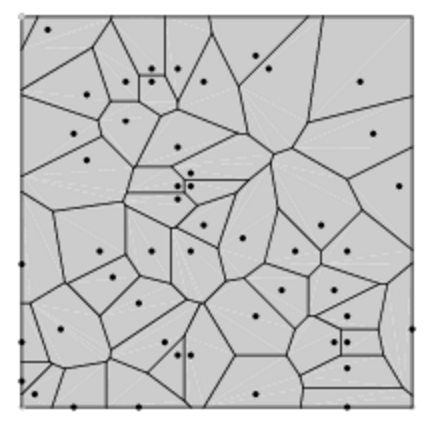
\includegraphics[width=6cm]{pics/diagramVoronoi.png}
	\caption{Diagram Voronoi}
	\label{fig:diagramVoronoi}
	\cite{diagram.voronoi}
\end{figure} 

\subsection{Contoh Aplikasi Diagram Voronoi}
\begin{enumerate}
\item Menggambarkan daerah yang didiami suatu pohon jika terdapat kumpulan pohon-pohon yang dilihat dari atas. \cite{voronoi.wiki}

\item Terdapat kumpulan pos ambulan di suatu kota, jika terdapat keadaan darurat di suatu tempat, dari pos manakah ambulan akan datang? \cite{voronoi.wiki}

\item Mengambil sampel jenis tanah di suatu daerah dan mengelompokkan jenis tanah masing-masing bagian berdasarkan sampel yang diambil. \cite{voronoi.wiki}
\end{enumerate}

\subsection{Macam-Macam Diagram Voronoi}
Menurut Okabe, dkk. \cite{spatial.tessellations} diagram Voronoi digeneralisasikan menjadi beberapa jenis sebagai berikut: 

\subsubsection{Weighted Voronoi Diagram}

Pada diagram Voronoi biasa secara implisit mengasumsikan bahwa setiap titik adalah identik (kecuali lokasinya) atau setiap titik memiliki bobot yang sama. Namun \textit{generator points} memiliki bobot yang berbeda yang mencerminkan sifat dari \textit{generator points} itu sendiri; sebagai contoh, ukuran populasi dari suatu pemukiman, jumlah fungsi-fungsi pada pusat perbelanjaan, jumlah emisi dari suatu polutan, ukuran dari sebuah atom pada suatu struktur kristal, dan lain-lain. 

Terdapat sekumpulan titik yang berbeda-beda, $\mathbb{P} = \left \{ p_{1},...,p_{n}\right \} \subset \mathbb{R}^{m} \left ( 2\leq n< \infty  \right ) \left ( A = P, S = \mathbb{R}^{m} \right )$ dan untuk masing-masing $p_{i}$ diberikan bobot yang sesuai dengan sifatnya. Kita representasikan bobot ini dengan sekumpulan parameter $\mathbb{W_{i}} = \left \{w_{i1},...,w_{in_{w}} \right \}$ (jika $n_{w} = 1$, kita tulis $w_{i}$ untuk $\mathbb{W_{i}}$). Dengan bobot ini kita definisikan jarak, $d_{w} \left(p,p_{i}\right)$, dari $p$ to $p_{i}$, disebut dengan sebuah \textit{weighted distance}. Daerah kekuasaan dari $p_{i}$ melalui $p_{j}$ dengan \textit{weighted distance}-nya ditulis dalam persamaan berikut:

\begin{equation} \label{eq1}
	Dom \left(p_{i},p_{j}\right)=\left \{p | d_{w}\left(p,p_{i}\right) \leq d_{w} \left(p,p_{j}\right) \right \}, j \neq i.
\end{equation}

dimana

\begin{equation} \label{eq2}
	V\left(p_{i}\right)=\bigcap_{i\in I_{n} \ \left {i \right }}^{} Dom \left(p_{i},p_{j}\right),
\end{equation}

dan $\mathbb{V} \left (P, d_{w}, \mathbb{R}^{m} \right ) = \mathbb{V}_{w} = \left \{ V \left(p_{1}\right),..., V\left(p_{n}\right ) \right \}$. $\mathbb{V}_{w}$ menghasilkan suatu \textit{generated Voronoi diagram}. Atau kita sebut $\mathbb{V}_{w}$ sebagai \textit{weighted Voronoi diagram} yang dihasilkan oleh $P$ dengan bobot $\left \{W_{1},...,W_{n} \right \}$, dan himpunan $V\left(p_{i}\right)$ merupakan \textit{weighted Voronoi region} yang berasosiasi dengan $p_{i}$. \cite{spatial.tessellations}

\textit{Weighted Voronoi diagram} merupakan pengembangan dari diagram Voronoi biasa. Berdasarkan definisi dari diagram Voronoi biasa, \textit{weighted Voronoi diagram} bisa didefinisikan sebagai berikut:

Terdapat $P = \left \{p_{1}, p_{2},...,p_{n}\right \}, 3 \leq n < \infty$ sebagai himpunan titik kontrol pada ruang Euclidean dua dimensi, $\lambda \left(i = 1,2,...,n\right)$ adalah bilangan asli, maka

\begin{equation} \label{eq3}
	V\left(p_{i},\lambda_{i}\right)=\left \{x \in V\left(p_{i},\lambda_{i}\right) | \frac{d\left (x,p_{i} \right )}{\lambda_{i}} \leq \frac{d\left (x,p_{j} \right )}{\lambda_{j}}, j = 1,2,...,n, j \neq i \right \}
\end{equation}

$d\left(p_{i},p_{j}\right)$ merepresentasikan jarak Euclidean di antara titik $p_{i}$ dan $p_{j}$, $p_{i} \neq p_{j}$, $i \neq j$, $i, j, \in \left \{1,2,...,n\right \}, x$ adalah sembarang titik di bidang tersebut.

Bidang dibagi menjadi $n$ bagian, \textit{weighted Voronoi diagram} adalah bidang yang dibagi oleh $V_{n}\left(p_{i},\lambda_{i}\right) \left(i = 1,2,...,n\right), \lambda_{i}$ adalah bobot dari $p_{i}$, seperti yang terlihat dalam gambar berikut, jumlah bobot dari titik.

\begin{figure}
	\centering
	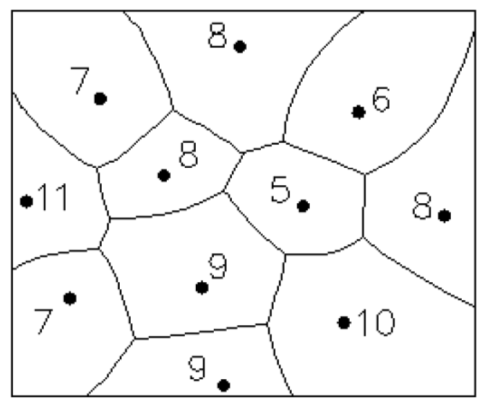
\includegraphics[width=6cm]{pics/weightedVoronoiDiagram.png}
	\caption{Weighted Voronoi Diagram}
	\label{fig:weightedVoronoiDiagram}
	\cite{substation}
\end{figure}

\textit{Weighted Voronoi graph} juga sesuai untuk segmentasi dari ruang. \textit{Weighted Voronoi diagram} digunakan untuk membagi ruang ketika terdapat perbedaan yang signifikan dari bobot untuk setiap titik. Ciri ini mengindikasikan bahwa bobot tersebut dapat digunakan untuk merefleksikan distribusi beban yang tidak sama dan efek-efek dari kapasitas dengan kadar yang berbeda dan kadar beban pada daerah yang dilayani oleh \textit{substation}.

Properti-properti dalam \textit{weighted Voronoi diagram}:

Dalam \textit{weighted Voronoi diagram}, $p_{i}, p_{j}$ merupakan dua \textit{occurrence elements} dengan sisi umum $l_{ij}$.

\begin{enumerate}
	\item Jika $\lambda_{i} = \lambda_{j}$, maka $l_{ij}$ adalah bagian dari garis vertikal dari segmen garis $p_{i}p_{j}$.
	\item Jika $\lambda_{i} \neq \lambda_{j}$, maka $l_{ij}$ adalah sebuah lingkaran atau lengkungan. Jika pusat dari garis lingkaran $l_{ij}$ adalah $O$, jari-jari $R$, koordinat $p_{i}$ adalah $\left(x_{i},y_{i}\right)$, koordinat dari $p_{j}$ adalah $\left(x_{j},y_{j}\right)$, $O, PI, PJ$ berada pada garis yang sama, dan
	\begin{enumerate}
		\item pusat koordinal adalah $\left(\frac{\lambda_{i}^{2} x_{j} - \lambda_{j}^{2} x_{i}}{\lambda_{i}^{2} - \lambda_{j}^{2}}, \frac{\lambda_{i}^{2} y_{j} - \lambda_{j}^{2} y_{i}}{\lambda_{i}^{2} - \lambda_{j}^{2}} \right)$;
		\item $R = \frac{\lambda_{i} \lambda_{j}}{| \lambda_{i}^{2} - \lambda_{j}^{2} |} d\left(p_{i},p_{j} \right)$;
		\item $d\left(O,p_{i} \right) = \frac{\lambda_{i}^{2}}{| \lambda_{i}^{2} - \lambda_{j}^{2} |} d\left(p_{i}, p_{j}\right)$, $d\left(O,p_{j} \right) = \frac{\lambda_{j}^{2}}{| \lambda_{j}^{2} - \lambda_{j}^{2} |} d\left(p_{i}, p_{j}\right)$
		\item $p_{i}, p_{j}$ adalah titik cermin dari lingkaran $O$
	\end{enumerate}
\end{enumerate} \cite{substation}

\subsubsection{Higher Order Voronoi Diagram}

Sebelum mengenal tentang \textit{higher order voronoi diagram}, kita perlu mengenal tentang \textit{first order voronoi diagram}. Terdapat sekumpulan titik $S$ pada bidang. Voronoi diagram dari $S$ adalah suatu dekomposisi dari suatu ruang ke dalam \textit{convex polygonal cells} (sel polihedral dalam dimensi yang lebih tinggi). Setiap titik $x$ dalam $S$ terkait dengan sebuah sel yang mengandung semua titik-titik dalam bidang tersebut yang lebih dekat dengan $x$ dari pada titik-titik lain dalam $S$. Sekumpulan sel kompleks ini adalah \textit{nearest neighbour decomposition.} \cite{hovd} 

\textit{Higher order voronoi diagram} mengekstend konsep diagram voronoi dengan mendefinisikan sel menggunakan $n$ \textit{nearest neighbour}. Sebagai contoh, jika $x$ dan $y$ adalah elemen yang berbeda dari $S$, maka terdapat suatu sekumpulan titik (yang kemungkinan besar kosong) yang mendefinisikan sebuah sel dalam diagram voronoi order kedua. tetangga terdekat dan tetangga terdekat kedua dari titik apapun dalam sel ini adalah $x$ dan $y$. Jumlah titik dalam $S$ yang mendefinisikan sebuah sel adalah order dari \textit{higher order voronoi diagram}.

Sebuah \textit{higher order voronoi diagram} (yang termasuk di dalamnya adalah \textit{first order voronoi diagram}) adalah sekumpulan sel yang membagi ruang. Bagaimanapun tidak seperti \textit{first order voronoi diagram}, \textit{dual} terhadap \textit{higher order voronoi diagram} tidak perlu membagi ruang. Sering terdapat kasus dimana segitiga dari \textit{higher order delaunay triangulation} akan memiliki persimpangan yang tidak kosong.

\subsubsection{Voronoi Diagrams with V-distances}

Voronoi diagram dapat digeneralisasi dengan jarak apapun selama jarak tersebut adalah V-distance. Jarak ini tidak harus jarak Euclidean. Seperti  \textit{multiplicatively weighted distance}, \textit{additively weighted distance}, \textit{compoundly weighted distance}, \textit{power distance} dan \textit{shortest-path distance}, yang mana bukan \textit{euclidean distance}, bisa membuat \textit{generalized voronoi diagram}. 

Voronoi diagram yang didefinisikan dengan Minkowski metriks dalam $R^m$. Minkowski (\textit{power}) metric dari suatu titik \textit{p} ke suatu titik $p_i$ dalam $R^m$ didefinisikan oleh

\begin{equation} \label{eqMinkowski}
d_L_p (p,p_i) = [\lambda_{j=1}^{m} | x_j - x_{ij} | ^ p]^{1/p}
\end{equation}

dimana ($x_1$,...,$x_m$) dan ($x_i1$,...,$x_im$) adalah koordinat Kartesian dari $p$ dan $p_i$, secara respektif. Secara random simbol $L_p$ adalah digunakan oleh metriks Minkowski, di mana $p$ merujuk pada derajat dari pangkat. Parameter $p$ berada pada range $1 \leq p < \infty$ . Jika $p = 1$, rumus \label{eqMinkowski} menjadi

\begin{equation} \label{manhattan}
d_L_1 (p, p_i) = \lambda_{j=1}^{m} | x_j - x_{ij} |
\end{equation} 

yang mana disebut dengan Manhattan metriks, \textit{city-block distance} atau \textit{taxi-cab distance}. Jika p=2, Minkowski metric adalah \textit{euclidean distance}. Jika $p = \infty$, Minkowski metric disebut dengan supremum metric atau dominance metric. \cite{spatial.tessellations}

\begin{figure}
	\centering
	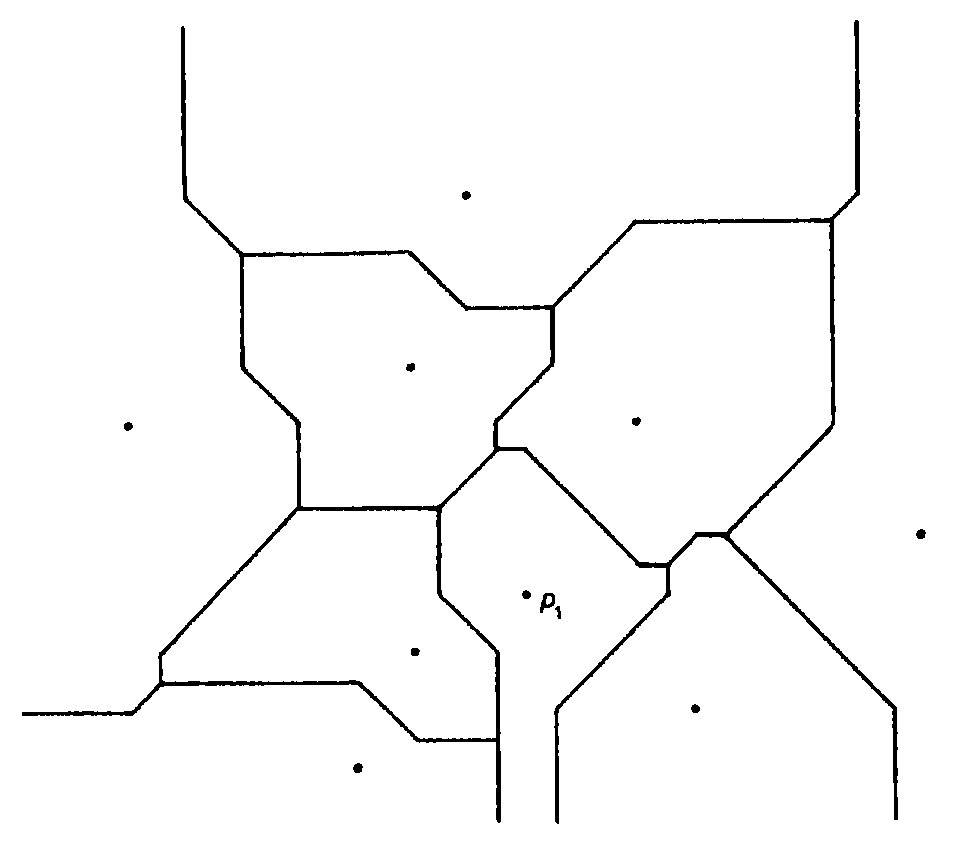
\includegraphics[width=10cm]{pics/manhattanVoronoiDiagram.png}
	\caption{Manhattan Voronoi Diagram}
	\label{fig:manhattanVoronoiDiagram}
	\cite{spatial.tessellations}
\end{figure}

\subsubsection{Network Voronoi Diagram}

Manhattan Voronoi diagram atau Karlsruhe Voronoi diagram berguna untuk menginvestigasi daerah yang dominan dalam sebuah \textit{grid street system} atau \textit{radial-circular street system}. Pada jalanan yang sesungguhnya, bahkan di Manhattan pun jalanan tidak sepenuhnya membentuk suatu grid. 

Terdapat \textit{planar geometric graph} G(N, L) terdiri dari sekumpulan nodes $N = {p_1,...,p_n,p_n+1,...,pl}$ dan sekumpulan links $L = {l_1,...,l_k}$ yang membentuk sebuah \textit{connected component}. Untuk menyederhanakan G(N,L) diasumsikan sebagai \textit{non-directed graph} (mengekstensi menjadi \textit{directed graph} tidak sulit). Pada G(N,L) mendefinisikan jarak dari sebuah titik p pada suatu link dalam L ke suatu node $p_i$ dalan N dengan jarak terpendeknya adalah dari p ke $p_i$.

\subsubsection{Voronoi Diagram for Moving Points}
Untuk jenis Voronoi diagram sebelumnya kita mengasumsikan bahwa lokasi dari generator adalah tetap sepanjang waktu. Dalam seksi ini diperhitungkan sebuah voronoi diagram yang dibuat dari sekumpulan titik yang selalu bergerak sepanjang waktu, atau secara umum merupakan sekumpulan titik yang lokasinya ditentukan oleh satu parameter.

\section{Macam-Macam Distances}

\subsection{Jarak Euclidean}
Jarak euclidean atau metriks euclidean adalah garis lurus biasa yang menghubungkan antara dua titik dalam \textit{euclidean space}. Dengan jarak ini \textit{euclidean space} menjadi \textit{metrics space}. \textit{Norm} (panjang) yang berhubungan dinamakan \textit{euclidean norm}. \textit{Euclidean distance} antara titik $p$ dan $q$ adalah panjang dari segmen garis yang menghubungkan mereka ($pq$).

Dalam koordinat kartesian, jika $p = (p_1, p_2, ..., p_n)$ dan $q = (q_1, q_2, ..., q_n)$ adalah dua titik dalam \textit{n}-ruang Euclidean, kemudian jarak (d) dari $p$ ke $q$, atau dari $q$ ke $p$ ditunjukkan oleh teorema Pythagoras:

\begin{equation} \label{euclidean}
	d(p, q) = d(q, p) = \sqrt{{\left (q_1 - p_1 \right )^2} + {\left (q_2 - p_2 \right )^2} + ... + {\left (q_n - p_n \right )^2}}
	= \sqrt{\sum_{i = 1}^{n} {(q_i - p_i)}^2}
\end{equation} 

Posisi dari sebuah titik dalam \textit{n}-ruang Euclidean adalah sebuah vektor Euclidean. Sehingga, $p$ dan $q$ adalah vektor-vektor Euclidean, yang dimulai dari sumber dari ruang, dan ujungnya mengarah pada dua titik. Euclidean \textit{norm} atau panjang Euclidean atau besar dari vektor menghitung panjang dari vektor:

\begin{equation}
	\left \| p \right \| = \sqrt{{p_1}^2 + {p_2}^2 + ... + {p_n}^2} = \sqrt{p.p}
\end{equation}

yang mana persamaan terakhir merupakan \textit{dot product}. \cite{euclidean.wiki}

\subsection{Chebyshev Distance}
\textit{Chebyshev distance} atau \textit{Tchebychev distance} adalah didefinisikan dalam metriks vektor dimana jarak antara 2 vektor adalah paling besar dari perbedaan mereka sepanjang dimensi koordinat apapun. 

	Disebut juga \textit{chessboard distance}. Dalam permainan catur jumlah pergerakan minimum dari king untuk berpindah dari satu kotak ke kotak lain setara dengan jarak Chebyshev antara titik pusat persegi ke titik pusat persegi lain jika sisi perseginya berukuran satu seperti yang direpresentasikan dalam koordinat spatial 2D dengan sumbu yang berada di tepi papan. Contohnya \textit{Chebyshev distance} antara f6 dan e2 adalah 4.
	
	Jarak Chebyshev antara dua vektor atau titik $p$ dan $q$, dengan standar koordinat $p_i$ dan $q_i$, adalah
	
\begin{equation}
	D_{Chebyshev}\left ( p,q \right ) := \underset{i}{max}\left ( \left | p_{i} - q_{i} \right | \right )
\end{equation}	 

Persamaan tersebut setara dengan limit dari metriks $L_p$:

\begin{equation}
\underset{k\rightarrow \infty }{lim} {\left ( \sum_{i = 1}^{n} {\left | p_i - q_i \right |}^{k}\right )}^{\frac{1}{k}}
\end{equation}

atau biasa disebut dengan metriks $L_\infty$.

	Secara matematika, jarak Chebyshev adalah metriks yang diinduksi oleh \textit{supremum norm} atau \textit{uniform norm}. Yang merupakan contoh dari metriks injektif.
	
	Dalam ruang dua dimensi, misalnya bidang, jika titik $p$ dan $q$ memiliki koordian Kartesian ($x_1, y_1$) dan ($x_2, y_2$), jarak Chebyshev-nya adalah
	
	\begin{equation}
	D_{Chess} = max \left ( \left | x_2 - x_1 \right |, \left | y_2 - y_1 \right | \right )
	\end{equation}
	
	Di bawah metriks tersebut, sebuah lingkaran dengan jari-jari $r$, yang mana kumpulan titik dengan jarak Chebyshev $r$ dari titik pusat, adalah sebuah persegi yang mana sisinya memiliki panjang $2r$ dan sejajar dengan sumbu koordinat $x$. \cite{chebyshev.wiki}

\subsection{Manhattan distance}
\textit{Manhattan distance} antara dua titik $x$ dan $y$ di ruang $n$ dimensi adalah jumlah jarak untuk masing-masing dimensi. Disebut Manhattan karena ini menggambarkan jarak suatu mobil yang berkendara dalam suatu kota (contoh Manhattan) dimana gedung-gedung ditata dalam blok-blok persegi dan jalan yang lurus memotong pada sudut kanan. L1 dan 1-\textit{norm distance} adalah deskripsi matematik untuk \textit{distance} ini.

\subsection{Mahalanobis Distance} 

Mahalonobis distance adalah jarak antara sebuah titik P dan sebuah distribusi D yang dikenalkan oleh P. C. Mahalonobis pada tahun 1936. Ini adalah generalisasi multi dimensi dari ide menghitung berapa banyak standar deviasi P dari rata-rata D. Jaraknya akan nol jika P berada pada rata-rata D, dan akan meningkat selama P menjauhi rata-rata dari D. Sepanjang setiap komponen utama dari sumbu, ini menghitung jumlah dari standar deviasi dari P ke rata-rata dari D. Jika setiap sumbu di skala ulang sehingga memiliki variansi unit, jarak Mahalonobis sebanding dengan jarak Euclidean standar pada ruang transformasi. Mahalonobis distance tidak memiliki unit dan skala nya tidak bervariasi, dan memperhitungkan hubungan dari data set. \cite{mahalanobis}

%-----------------------------------------------------------------------------%
%\section{Metode Perhitungan}\label{sec:metodePerhitungan}
%-----------------------------------------------------------------------------%

%-----------------------------------------------------------------------------%
\section{Menentukan Jumlah \textit{Station} Baru}\label{sec:jumlahStationBaru}
%-----------------------------------------------------------------------------%

Dalam paper Xiaojun dkk, metode yang digunakan untuk menghitung kuantitas dan kapasitas dari \textit{substation} adalah menghitung jumlah \textit{stations} baru, menghitung kapasitas dari \textit{station} baru, dan menggunakan \textit{weighted Voronoi diagram}.

Berdasarkan jumlah beban dari target, kapasitas dari \textit{station} saat ini dan himpunan kapasitas dari calon \textit{substation}, jumlah maksimum dari $n\left(max\right)$ dan jumlah minimum dari $n\left(min\right)$ dan jumlah \textit{substation} baru (\textit{n}) bisa ditentukan dengan persamaan \ref{eq4} dan \ref{eq5}, yang mana di bawah kondisi \textit{power supply}.

\begin{equation} \label{eq4}
	n_{max} = \frac{\sum W - \sum P}{\left ( S_{e} \right)_{min} cos \varphi} + \eta
\end{equation}

\begin{equation} \label{eq5}
	n_{min} = \frac{\sum W - \sum P}{\left ( S_{e} \right)_{max} cos \phi}
\end{equation}

\begin{figure}
	\centering
	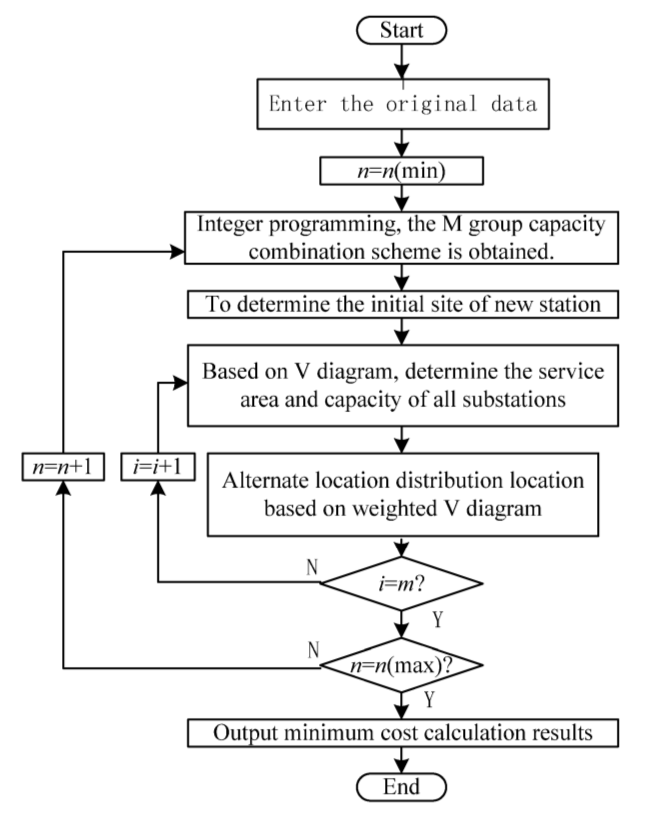
\includegraphics[width=10cm]{pics/substationPlanning.png}
	\caption{Flow Chart dari Substation Planning}
	\label{fig:substationPlanning}
	\cite{substation}
\end{figure}

$\sum W$ adalah jumlah muatan aktif dari seluruh muatan; $\sum P$ adalah jumlah kapasitas daya aktif dari \textit{transformer substation} dalam tahun (termasuk ekspansi dari kapasitas \textit{station} saat ini); $S\left(Se\right)_{max} = max\left \{S_{i}e \left(S_{i}\right) | S_{i} \in Q \right \}$ adalah nilai maksimum kapasitas ekonomi (kapasitas x \textit{load ratio}) dalam tipe kandidat untuk \textit{substation}; $\left(Se\right)_{min}$ adalah kapasitas ekonomi minimum dari tipe kandidat dari \textit{substation}; $\eta$ adalah \textit{relaxation factor}.

%-----------------------------------------------------------------------------%
%\subsection{Menentukan Kapasitas dari Substation Baru}\label{sec:kapasitasStationBaru}
%%-----------------------------------------------------------------------------%
%
%Jika jumlah dari \textit{station} baru adalah $n$, kita dapat menentukan m grup kombinasi dari kapasitas \textit{station} baru berdasarkan kapasitas dari \textit{transformer substation} yang baru dan kapasitas dari \textit{station} saat ini pada tahun yang telah ditargetkan. Dapat dibentuk model matematika seperti berikut:
%
%\begin{figure}
%	\centering
%	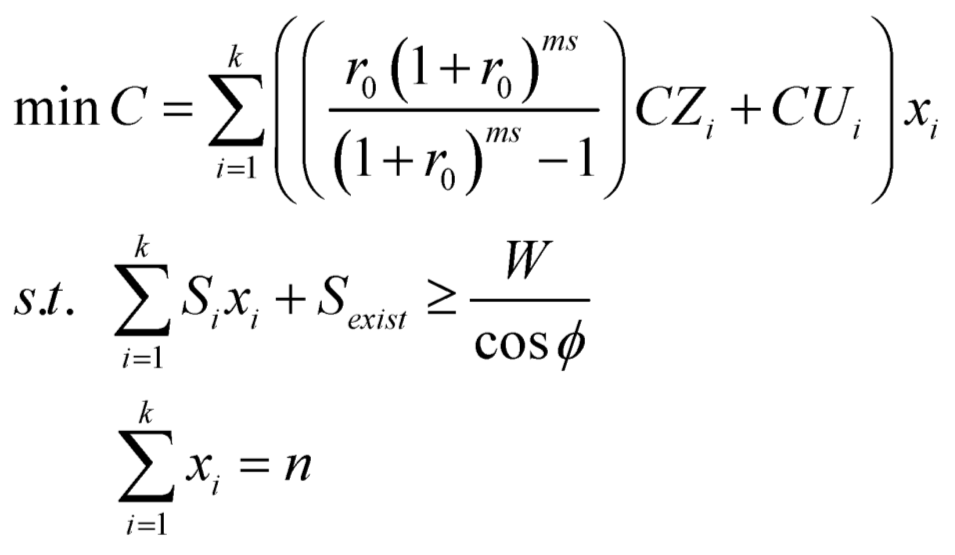
\includegraphics[width=9cm]{pics/formula.png}
%	\label{eq6}
%	\cite{substation}
%\end{figure}
%
%$k$ adalah jumlah dari tipe kandidat \textit{transformer substation}; $CZ_{i}$ adalah biaya investasi dari $i$ kandidat tipe \textit{transformer substation}; 

%-----------------------------------------------------------------------------%
\section{Hotspot}\label{sec:hotspot}
%-----------------------------------------------------------------------------%

%- Menghitung kapasitas suatu hotspot (kapasitas ini bisa kekuatan si hotspot atau luas area jangkauannya)

%- penempatan hotspot di suatu ruang terbuka
% Untuk open area tinggal ngitung 100m jari2 dari pusat (atau diameter?). kalo misal UI dianggap open area, berarti bikin lingkaran2 per 100 m, (minus danau dan hutan)

\textit{Wi-Fi hotspot} adalah \textit{wireless access point} yang menyediakan jaringan atau akses internet untuk perangkat \textit{mobile} seperti \textit{laptop} atau \textit{smartphone}, yang biasanya terdapat di tempat-tempat umum.  

Wi-Fi digunakan untuk menyediakan akses internet untuk perangkat yang berada dalam jangkauan dari jaringan nirkabel yang terhubung dengan internet. Cakupan dari satu atau lebih \textit{hotspot-hotspot} yang saling berhubungan bisa diperluas dari suatu area yang hanya seluas sebuah kamar hingga seluas beberapa kilometer persegi. Cakupan dalam daerah yang lebih luas membutuhkan sekumpulan \textit{access point} dengan cakupan yang saling tumpang tindih. Contohnya teknologi \textit{public outdoor Wi-Fi} yang telah berhasil diimplementasikan dalam \textit{wireless mesh network}.

\textit{Wireless Mesh Network} (WMN) adalah jaringan komunikasi yang terdiri dari \textit{radio nodes} yang terorganisir dalam \textit{mesh topology}. WMN terdiri dari \textit{mesh clients}, \textit{mesh routers} dan \textit{gateways}. 

\textit{Mesh clients} merupakan perangkat yang menggunakan jaringan nirkabel tersebut, seperti laptop, telefon seluler, dan perangkat-perangkat nirkabel lainnya. \textit{Mesh routers} digunakan untuk meneruskan arus baik dari atau menuju ke \textit{gateways}. \textit{Router} bisa terhubung atau tidak terhubung ke internet. 

\section{GIS}
\textit{still don't know why we need this}

\section{Tools}
Terdapat beberapa \textit{tools} yang dapat digunakan untuk mengimplementasikan \textit{weighted Voronoi diagram}, diantaranya: R studio, ArcGIS, WVD18, java library, dan lain-lain.

\subsection{R Studio}

%R studio 
%https://www.stat.auckland.ac.nz/~paul/Reports/VoronoiTreemap/voronoiTreeMap.html

RStudio adalah Integrated Development Environment (IDE) untuk R yang didalamnya terdapat console, syntax-highlighting editor yang mendukung eksekusi kode secara langsung, melakukan plotting, melihat history, debugging, dan manajemen \textit{workspace}.

Kelebihan dari tools ini adalah dapat melakukan perhitungan voronoi diagram serta melakukan \textit{plotting} dari diagram.

\subsection{ArcGIS}
ArcGIS adalah \textit{platform} yang digunakan untuk melakukan pemetaan dan analisis. ArcGIS dapat melakukan untuk melakukan analisis spasial, pemetaan dan visualisasi, menggambarkan GIS 3D, \textit{real time} GIS, perbandingan dan \textit{remote sensing}, serta pengumpulan dan managemen data. \cite{arcgis}

\subsection{OpenVoronoi}

OpenVoronoi adalah suatu tools yang menghitung voronoi diagram 2D untuk titik, garis lurus dan garis lengkung. Kekurangan dari tools ini adalah belum mengeluarkan output berupa gambar. Perlu ditambahkan beberapa program untuk menghasilkan gambar diagram voronoinya. \cite{open.voronoi}

\subsection{Java Library: Power Voronoi Diagram}

Power Voronoi Diagram merupakan Java Library yang menghitung suatu weighted voronoi diagram yang disebut Power Diagram. Perbedaan utama dengan voronoi diagram biasa adalah kemungkinan untuk memberikan bobot positif untuk setiap situs yang akan mempengaruhi sel-sel voronoi yang berkaitan. Jika bobot tersebut diberi nilai nol, maka hasilnya merupakan diagram voronoi biasa. \cite{power.voronoi.diagram}

Java Library ini hanya melakukan perhitungan dan pembuatan diagram voronoi tanpa melakukan penggambaran diagramnya.

%-----------------------------------------------------------------------------%
\section{Peta Kampus Universitas Indonesia}\label{sec:petaUI}
%-----------------------------------------------------------------------------%

Kampus Universitas Indonesia Depok memiliki luas 320 hektar yang terdiri dari 75 persen area hijau seperti hutan dan danau \cite{ui}. 25 persennya terdiri dari fakultas-fakultas dan jalan yang menghubungkan antarfakultas. 

Selain fakultas, dalam area kampus UI Depok juga terdapat fasilitas umum seperti perpustakaan, stasiun, asrama, rektorat, dan lain-lain.

\begin{figure}
	\centering
	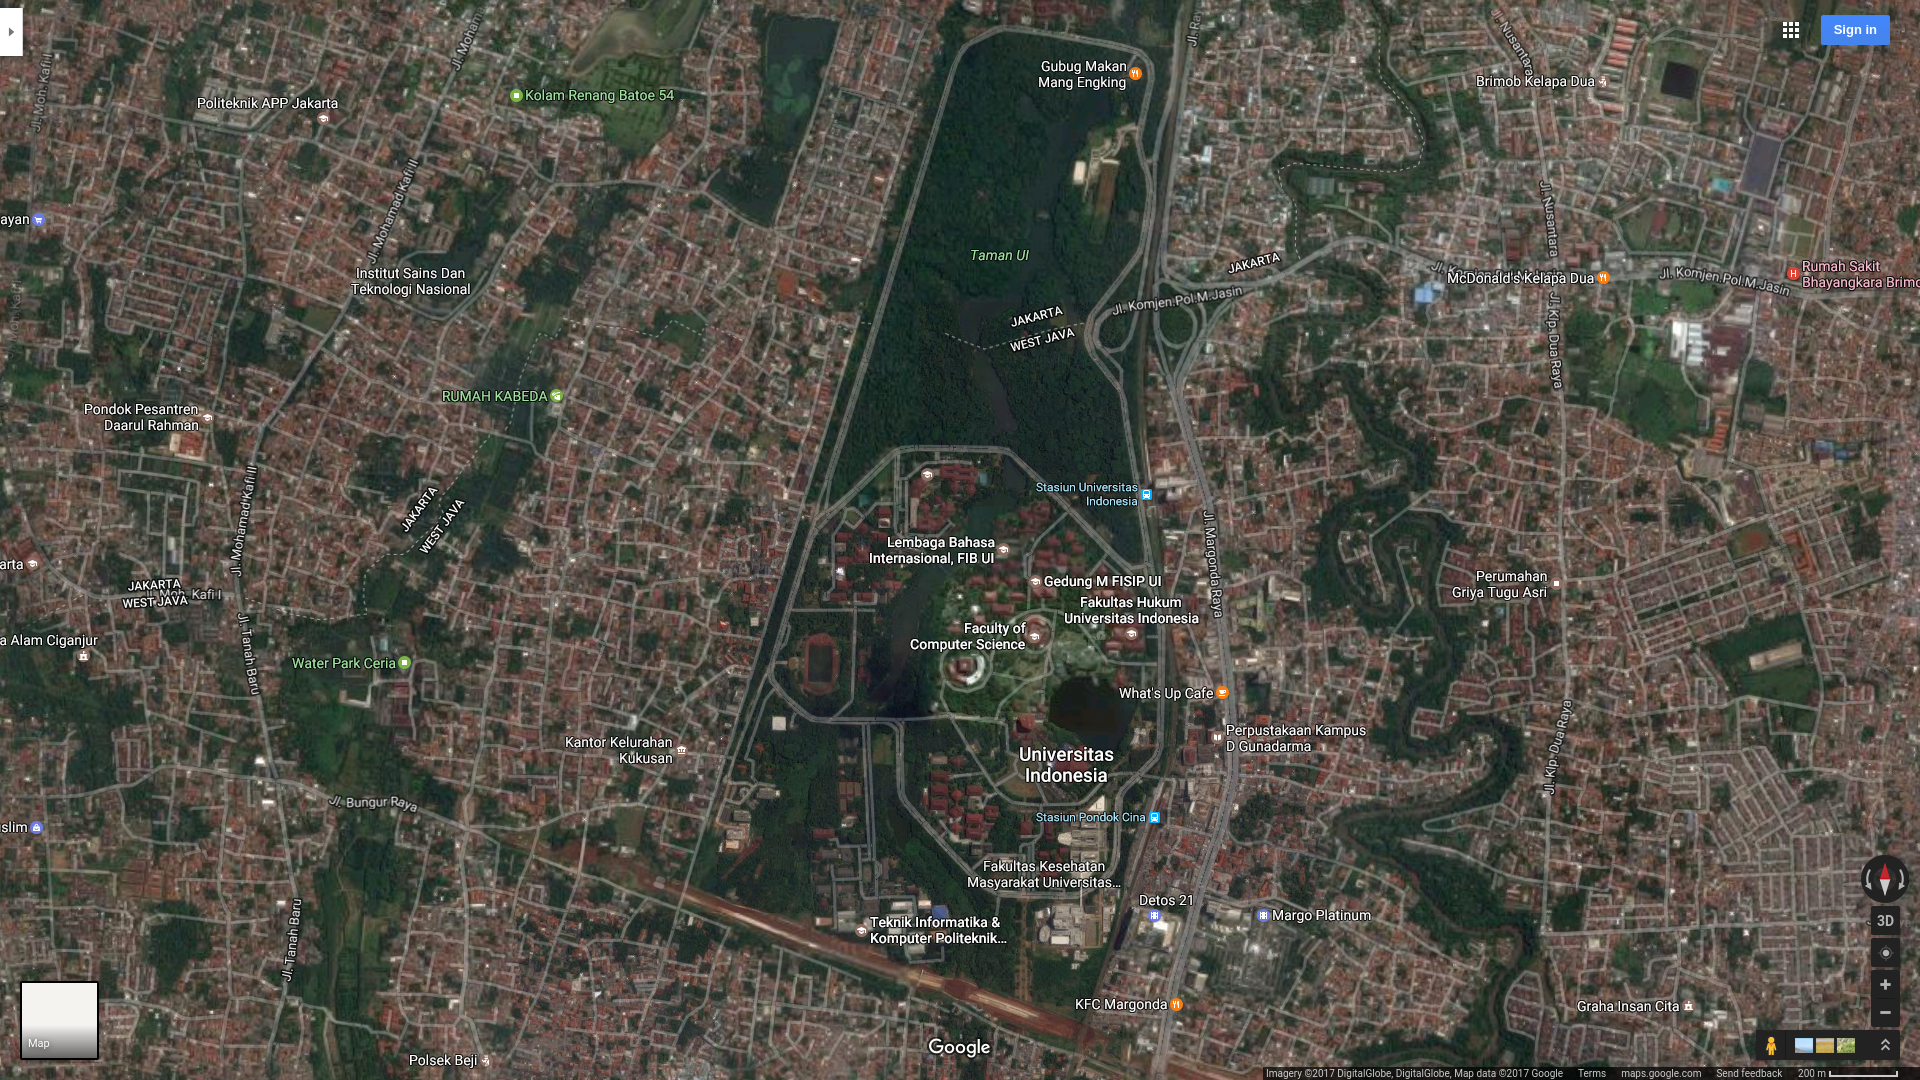
\includegraphics[width=14cm]{pics/ui-map.png}
	\caption{Peta Kampus Universitas Indonesia Depok}
	\label{fig:UImap}
	\cite{ui.map}
\end{figure}

Universitas Indonesia terdiri atas 47.641 mahasiswa (tahun 2015) yang tersebar dalam 14 fakultas yang tergolong dalam tiga rumpun, yaitu Rumpun Ilmu Kesehatan (RIK), Rumpun Sains-Teknologi (Saintek), dan Rumpun Sosial-Humaniora (Soshum). \cite{ui.wiki}

Yang termasuk dalam Rumpun Ilmu Kesehatan adalah:
\begin{itemize}
 \item Fakultas Kedokteran
 \item Fakultas Kedokteran Gigi
 \item Fakultas Farmasi
 \item Fakultas Kesehatan Masyarakat
 \item Fakultas Ilmu Keperawatan
\end{itemize}

Rumpun Sains-Teknologi:
\begin{itemize}
\item Fakultas Matematika dan Ilmu Pengetahuan Alam
\item Fakultas Teknik
\item Fakultas Ilmu Komputer
\end{itemize}

Rumpun Sosial-Humaniora:
\begin{itemize}
\item Fakultas Hukum
\item Fakultas Ekonomi dan Bisnis
\item Fakultas Ilmu Pengetahuan Budaya
\item Fakultas Psikologi
\item Fakultas Ilmu Sosial dan Ilmu Politik
\item Fakultas Ilmu Administrasi
\end{itemize}

\section{WiFi 101}

WiFi adalah sebuah teknologi untuk \textit{wireless local area networking} dengan \textit{device} yang menggunakan standar IEEE 802.11. WiFi adalah merek dagang dari Wi-Fi Alliance, yang membatasi penggunaan term WiFi Certified dengan produk yang telah menyelesaikan tes sertifikasi \textit{interoperabilility}. \cite{wifi}

\textit{Device} yang bisa menggunakan teknologi WiFi diantaranya \textit{personal computer}, \textit{video-game console}, \textit{handphone} dan \textit{tablet}, kamera digital, \textit{smart} TV, \textit{digital audio player}, dan printer modern. \textit{Device} yang kompatibel dengan WiFi bisa terhubung dengan internet melalui WLAN dan \textit{wireless access point}. Sebuah akses poin atau \textit{hotspot} memiliki jarak sekitar 20 meter untuk \textit{indoor} dan jaraknya lebih jauh untuk \textit{outdoor}. Jangkauan \textit{hotspot} bisa sekecil satu ruangan dengan dinding yang memblokir gelombang radio, dan bisa seluas beberapa kilometer persegi yang bisa dicapai dengan menggunakan beberapa \textit{overlapping access point}.

WiFi biasanya menggunakan frekuensi radio 2.4 \textit{gigahertz} (12 cm) UHF dan 5.8 \textit{gigahertz} (5 cm) SHF ISM. Siapapun yang berada dalam jangkauan tersebut dan menggunakan \textit{modem wireless} bisa mengakses jaringan tersebut. Karena hal itu, WiFi lebih rentan untuk diserang (yang disebut dengan \textit{eavesdropping}) dibandingkan dengan jaringan kabel.
%--------------------------------------------------------------------------a---
\chapter{\babTiga}
%-----------------------------------------------------------------------------%

Bab ini menjelaskan tentang metode penelitian yang digunakan beserta langkah-langkahnya.

Berdasarkan latar belakang masalah, rumusan masalah, tujuan penelitian, dan ruang lingkup pengerjaan yang telah dibahas pada bab satu, metodologi penelitian yang digunakan dalam penelitian ini adalah sebagai berikut.

\section{Studi Literatur}
Pada tahap ini dilakukan studi literatur tentang teori-teori dan metode yang mendukung penelitian ini. Studi literatur yang dilakukan adalah mempelajari tentang Voronoi Diagram dan implementasinya, mempelajari lebih dalam tentang Weighted Voronoi Diagram dan research tentangnya, \textit{tools} dan aplikasi yang dapat digunakan untuk mengimplementasikan Weighted Voronoi Diagram, macam-macam \textit{distance}, \textit{hotspot} dan Wi-Fi, serta mempelajari tentang \textit{hotspot} di Universitas Indonesia.

\subsection{Diagram Voronoi yang Digunakan}
Setelah melakukan riset terhadap jenis diagram Voronoi yang ada, ditentukan bahwa diagram Voronoi yang digunakan dalam penelitian ini adalah \textit{weighted Voronoi diagram}. Hal ini dikarenakan \textit{todo alasan} 

\subsection{Distance yang Digunakan}
Setelah melakukan riset mengenai jenis \textit{distance} yang digunakan dalam penelitian ini, ditentukan bahwa \textit{distance} yang digunakan adalah Euclidean \textit{distance}. Hal ini dikarenakan jarak Euclidean merupakan jenis jarak yang paling sederhana.

\subsection{Pemetaan Weighted Voronoi Diagram dan Hotspot}
Dalam penelitian ini, \textit{weight} dalam \textit{weighted Voronoi diagram} digambarkan dengan kekuatan sinyal dan bandwidth dari hotspot.

\section{Research Tools}
Untuk menggambarkan Weighted Voronoi Diagram diperlukan suatu \textit{tools} atau aplikasi. Terdapat berbagai macam \textit{tools} yang dapat digunakan untuk menggambarkan Weighted Voronoi Diagram. Setiap \textit{tools} yang ada memiliki fungsi dan penggunaannya masing-masing. Berikut merupakan hasil riset untuk \textit{tools} yang telah dilakukan.

\begin{table}[H]
\centering
\caption{Hasil Riset \textit{Tools}}
\label{research-tools}
\scalebox{0.7}{%
\begin{tabular}{|l|c|c|c|}
\hline
 & \multicolumn{1}{l|}{Menghitung Diagram Voronoi} & \multicolumn{1}{l|}{Menggambar Diagram Voronoi} & \multicolumn{1}{l|}{Menggambar Peta} \\ \hline
R Studio & v & v & v \\ \hline
Open Voronoi & v &  &  \\ \hline
Power Voronoi Diagram & v &  &  \\ \hline
ArcGIS &  & v & v \\ \hline
\end{tabular}}
\end{table}

Setelah melakukan riset untuk \textit{tools} yang akan digunakan dalam penelitian ini, ditentukan bahwa \textit{tools} yang akan digunakan adalah RStudio. RStudio dipilih karena selain dapat melakukan perhitungan diagram voronoi, dalam RStudio juga bisa melakukan \textit{plotting} untuk diagram dengan \textit{output} berupa gambar .png.

\section{Data}
Untuk melakukan penelitian ini diperlukan informasi tentang lokasi dari \textit{access point} \textit{hotspot} yang ada di Universitas Indonesia. Untuk mendapatkan informasi tersebut perlu menghubungi Direktorat Sistem & Teknologi Informasi (DSTI) Universitas Indonesia. DSTI merupakan lembaga yang bertanggung jawab untuk mengelola sarana dan prasarana yang berhubungan dengan Teknologi Informasi di Universitas Indonesia. 

Data yang digunakan dalam penelitian ini adalah data lokasi dari \textit{access point} yang ada di Universitas Indonesia. Data yang didapat dari DSTI {\ui} masih berupa data mentah. Data tersebut harus diolah dulu untuk bisa digunakan dalam penelitian ini.

\section{Implementasi Dasar}
Implementasi dasar yang akan dilakukan adalah memetakan data yang didapat dari DSTI ke dalam peta {\ui}. Setiap satu lokasi \textit{access point} digambarkan sebagai satu titik dalam peta. Penempatan dari setiap titik sesuai dengan koordinat yang telah didapat dari pengolahan data.

\section{Penambahan Bobot dan Jangkauan}
Masing-masing titik diberikan bobotnya sebagai bobot dari Weighted Voronoi Diagram. Bobot ini sesuai dengan beban dan bandwidth dari setiap \textit{access point}. Selain bobot juga ditambahkan jangkauan dari setiap \textit{access point} yang berupa lingkaran-lingkaran yang berpusat pada titik tersebut. Berdasarkan titik dan bobotnya, kemudian digambarkan diagram voronoi untuk setiap titik.

\section{Modifikasi Implementasi dan Data}
Dalam peta, titik merupakan gambaran dari lokasi \textit{access point}. Lingkaran merupakan gambaran dari jangkauan suatu \textit{access point}. Bobot dari suatu titik merupakan penggambaran dari beban kapasitas yang harus di-\textit{cover} oleh satu \textit{access point}. Diagram Voronoi berperan sebagai penggambaran dari lokasi yang harus dijangkau oleh suatu \textit{access point}. 

Kondisi ideal adalah kondisi dimana setiap daerah dalam peta berada di dalam lingkaran. Yang berarti setiap daerah mendapatkan sinyal \textit{hotspot}. Kondisi inilah yang akan dicapai dalam penelitian ini. 

\begin{figure}
	\centering
	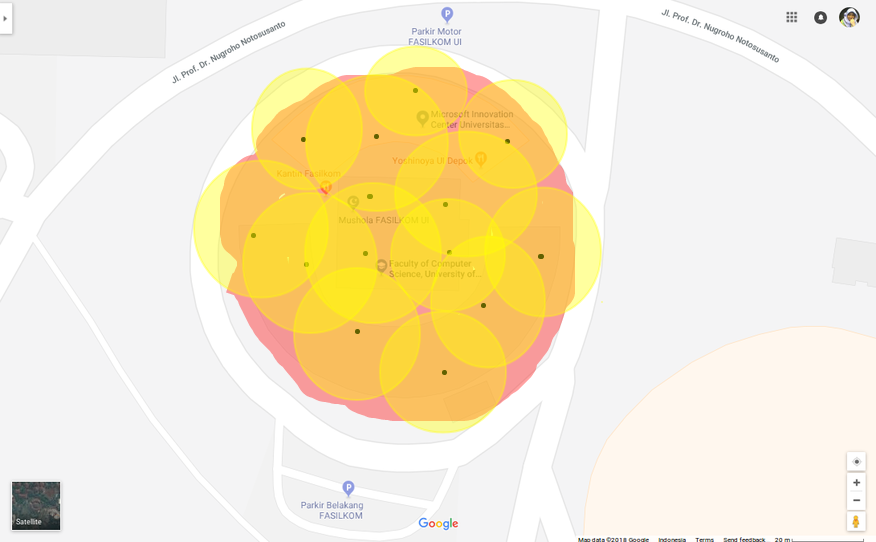
\includegraphics[width=10cm]{pics/fasilkom-demand-coverage.png}
	\caption{Kondisi Ideal}
	\label{fig:kondisiIdeal}
\end{figure}

Kondisi yang tidak ideal adalah kondisi di mana terdapat daerah dalam peta yang tidak berada di dalam lingkaran. Hal ini berarti daerah tersebut tidak mendapatkan sinyal Wi-Fi. Untuk itu perlu ditambahkan satu titik baru di daerah di luar lingkaran sehingga daerah tersebut mendapatkan sinyal Wi-Fi. 

\begin{figure}
	\centering
	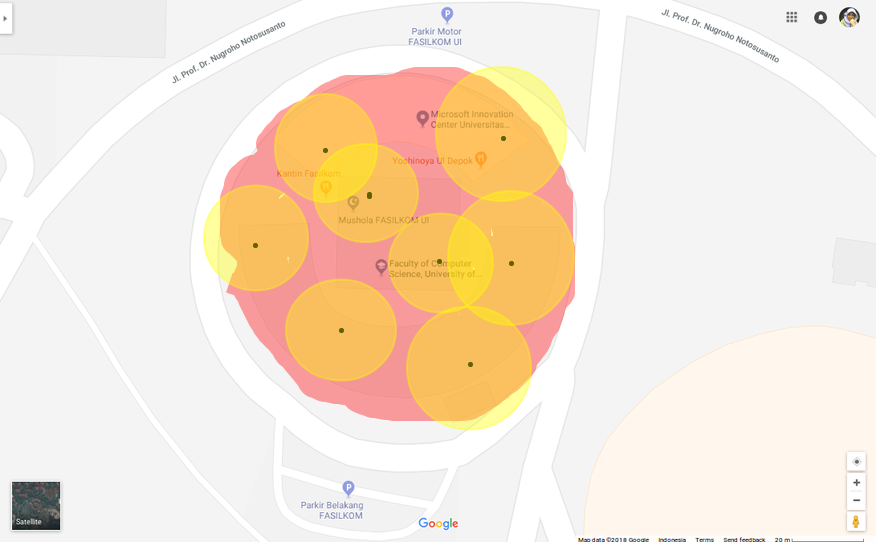
\includegraphics[width=10cm]{pics/fasilkom-demand-coverage-minus.png}
	\caption{Kondisi Tidak Ideal}
	\label{fig:kondisiTidakIdeal}
\end{figure}

Proses penambahan titik ini dilakukan secara iteratif sehingga setiap daerah berada dalam jangkauan sinyal Wi-Fi atau berada di dalam lingkaran.

\begin{figure}
	\centering
	\includegraphics[width=14cm]{pics/tahapanPenelitian.png}
	\caption{Tahapan Penelitian}
	\label{fig:tahapanPenelitian}
\end{figure}

\section{Pemetaan dari Paper}

n max = jumlah maksimal station baru = jumlah maksimal \textit{hotspot} device

n min = jumlah minimal station baru = jumlah minimal \textit{hotspot} device

n = jumlah station baru = jumlah \textit{hotspot} device baru

sigma W = total active load =

sigma P = total active power kapasitas ekonomi = 

Se max = nilai maksimum dari kapasitas ekonomi (kapasitas x rasio load) =

Se min = kapasitas ekonomi minimum dari tipe kandidat dari substation
eta = relaxation faktor = 

M = jumlah grup dari skema kombinasi kapasitas =  

m = same with M? =

k = jumlah tipe kandidat substation = jumlah tipe kandidat \textit{hotspot} device

CZi = cost investasi dari i tipe kandidat transformer substation = 

CUi = cost operasi tahunan dari i tipe kandidat dari transformer 

substation =

r0 = diskon rate = 

ms = periode depresiasi dari substation = 

xi = jumlah dari i tipe kandidat konstruksi transformer = 

Si = kapasitas dari i tipe kandidat substation (load rate sudah di 

peretimbangkan) =

Sgxist = kapasitas existing station (load rate sudah dipertimbangkan) = 

W = total load = 

cos phi = power factor = 

\section{\textit{Distance} yang Digunakan}
Dalam penelitian ini menggunakan Euclidean \textit{distance} karena Euclidean merupakan \textit{distance} yang paling sederhana. 

\section{Evaluasi keberhasilan}
Parameter keberhasilan dalam penelitian ini ada dua, yaitu menggambarkan Weighted Voronoi Diagram dari lokasi-lokasi \textit{access point} di {\ui} beserta jangkauannya dan mendapatkan lokasi-lokasi \textit{access point} baru sehingga setiap daerah mendapatkan sinyal Wi-Fi.

%\section{Desain dan Implementasi}
%\subsection{Desain Sistem}

%Desain dari sistem yang akan dibuat adalah sebagai berikut:

%\begin{enumerate}
%\item Pemetaan lokasi hotspot

%Lokasi hotspot saat ini dipetakan ke dalam peta 

%\item Penggambaran diagram voronoi

%Digambarkan weighted voronoi diagram dari persebaran hotspot saat ini, dengan kekuatan signal dari hotspot sebagai weight.

%\item Dilakukan pengecekan untuk setiap perbatasan dua atau lebih diagram. Pengecekan yang dilakukan adalah kekuatan signal dan bandwidth (terdapat threshold minimalnya)

%\item Kalau kurang dari threshold maka perlu ditambah device baru di titik tersebut
%\item Berarti satu iterasi itu meliputi setiap dua atau lebih diagram.  Maksudnya dia akan mencari di setiap perbatasan mana saja yg kurang kapasitasnya.
%\item Setelah diketahui titik-titiknya, kemudian digambarkan device baru di titik-titik tersebut. (pemetaan lokasi hotspot baru)
%\item Setelah itu kembali ke tahap penggambaran diagram voronoi, dan seterusnya sampai tujuan tercapai (tidak ada titik yg di bawah threshold signal dan bandwidth minimal)
%\end{enumerate}

%\begin{figure}
%	\centering
%	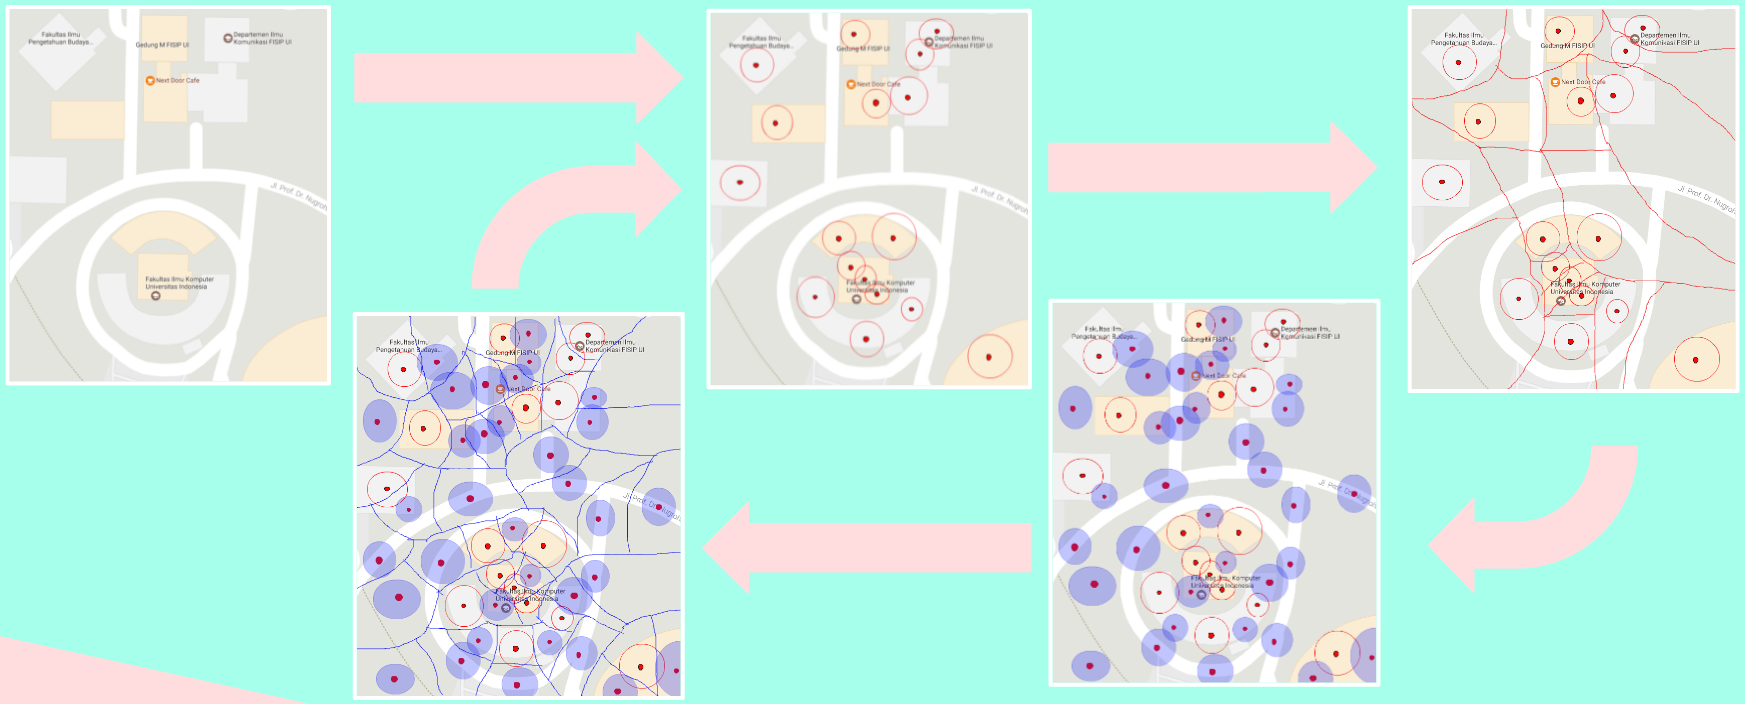
\includegraphics[width=14cm]{pics/desainProses.png}
%	\caption{Desain Proses}
%	\label{fig:desainProses}
%\end{figure}

%\subsection{Desain Interaksi}

%Desain interaksi dari sistem yang akan dibuat adalah sebagai berikut:

%\begin{enumerate}
%	\item User memasukkan peta, jumlah titik (hotspot) dan koordinat dari masing-masing titik.
%	\item Ditampilkan hasil pemetaan titik-titik hotspot ke dalam peta.
%	\item Digambarkan weighted voronoi diagram dari kumpulan titik-titik tersebut.
%	\item Dilakukan penghitungan kekuatan signal dan bandwidth untuk setiap perbatasan diagram.
%	\item Menampilkan lokasi dari calon hotspot baru.
%\end{enumerate}



%%-----------------------------------------------------------------------------%
%\section{Studi Literatur}
%-----------------------------------------------------------------------------%
%

%
%%-----------------------------------------------------------------------------%
%\section{Desain dan Implementasi}
%-----------------------------------------------------------------------------%
%
%Pada tahap ini akan dilakukan perancangan sistem yang akan dibuat, serta tahapan implementasi dari sistem tersebut.
%
%\subsection{Pemetaan Lokasi}
%
%Pada tahap ini akan dilakukan pemetaan lokasi-lokasi dari fasilitas umum yang akan dianalisis. Pemetaan akan dilakukan dengan menggunakan R Software, yaitu RStudio. Dalam peta yang dibuat terdapat informasi tentang lokasi-lokasi dari fasilitas umum yang akan dianalisis. Data tersebut digambarkan dalam format vektor, yaitu dalam bentuk \textit{area} untuk peta dari daerah yang akan dianalisis, serta bentuk \textit{point} untuk lokasi-lokasi dari fasilitas umum. %perlu tambah teori tentang RStudio?
%
%\subsection{Penggambaran Diagram Voronoi}
%
%Pada tahap ini akan dilakukan penggambaran diagram Voronoi pada peta yang telah dipetakan lokasi-lokasi fasilitas umum yang akan dianalisis. Penggambaran diagram Voronoi dilakukan dengan menggunakan Wolfram Alpha. Koordinat dari lokasi-lokasi pada peta di dalam tahap sebelumnya masing-masing  dipetakan ke Wolfram Alpha dan dibuat diagram Voronoi-nya menggunakan perintah VoronoiDiagram yang terdapat dalam paket ComputationalGeometry.  %teori tentang wolfram juga?
%
%Diagram Voronoi yang dihasilkan dari Wolfram Alpha kemudian dipetakan kembali ke dalam peta pada R Software. Hal ini dilakukan agar ruang lingkup atau daerah cakupan dari masing-masing lokasi fasilitas umum bisa terlihat dengan jelas.
%
%%Okay disini kalimat-kalimat kasarnya dulu. Jadi tuh desainnya apa ya? desain programnya? Kan aku mau bikin sesuatu yang bisa digunakan untuk mencari lokasi optimal untuk fasilitas umum. Nyari lokasinya pake apa? Pertama kan udah ada info tentang lokasi-lokasi fasilitas umum itu (udah ada peta yang isinya lokasi-lokasi fasilitas umum). Terus digambarlah diagram Voronoi di peta itu, jadi tau cakupan dari masing-masing fasilitas umum itu. 
%
%\subsection{Penambahan Data Spasial}
%
%Pada tahap ini akan dilakukan penambahan informasi-informasi yang terkait dengan data spasial untuk daerah dalam peta. Informasi-informasi yang ditambahkan diantaranya:
%
%\begin{itemize}
%\item[-] Data kepadatan penduduk di daerah tersebut
%\item[-] Tingkat permintaan akan fasilitas umum pada daerah tersebut
%\end{itemize}
%
%Informasi tersebut kemudian dipetakan ke dalam peta pada R Software dengan format vektor dalam bentuk \textit{area} dengan warna tertentu yang berbeda dengan warna peta dasar dan berbeda untuk masing-masing informasi. 
%
%Untuk tingkat kepadatan penduduk yang lebih tinggi akan dibuat dengan warna yang lebih pekat. Begitu juga untuk tingkat permintaan akan fasilitas umum pada daerah tersebut.
%
%%Kemudian mencari data untuk:
%
%- Kapasitas masing-masing fasilitas umum
%- Kepadatan penduduk di daerah tersebut
%- Demand untuk fasilitas umum tersebut di daerah itu
%
%\subsection{Perhitungan Kebutuhan Fasilitas Umum}
%
%Pada tahap ini akan dilakukan perhitungan jumlah kebutuhan fasilitas umum untuk suatu daerah dalam satu waktu. Perhitungan dilakukan dengan cara mengalikan jumlah penduduk dengan tingkat permintaan untuk fasilitas umum yang akan dianalisis. Hasil tersebut kemudian dibandingkan dengan kapasitas masing-masing fasilitas umum sehingga dapat diketahui apakah fasilitas umum tersebut bisa mencukupi kebutuhan di lingkungan tersebut.
%
%Tingkat kebutuhan akan fasilitas umum yang dinamis, membuat analisis mengenai lokasi yang optimal dari fasilitas umum ini perlu dilakukan sesuai dengan perubahan penduduk dan tingkat kebutuhan akan fasilitas umum tersebut.
%
%%Setelah mendapatkan data untuk daerah tersebut, kemudian bisa dihitung dengan kapasitas sekian, jumlah penduduk kali demand untuk daerah itu berapa, maka tempat itu cukup ga untuk melayani permintaan? Mungkin ga sekedar permintaan di satu waktu ya, karna untuk setiap waktu kan pasti jumlah permintaannya beda-beda.
%
%%Kalo rumah sakit contohnya, mungkin bisa dicari masa-masa orang sakit tuh kapan aja. Misalnya pas musim pancaroba, atau pas musim hujan. 
%
%%Tapi kan informasi tentang rate itu pasti per daerah ya, kaya misal perkabupaten atau perkecamatan. Sedangkan cakupan dari diagram Voronoi itu random, ga berbatas kecamatan atau kabupaten. Jadi harus ngitung dulu rata-rata dari tempat itu. Kaya misal satu daerah Voronoi itu gabungan dari 3 kecamatan, kan brarti ada porsi untuk masing2 kecamatannya seberapa luas. Jumlah penduduk dibagian itu berapa. Terus dicari rata2nya. Nah rata2 ini ga serta merta dibagi tiga, tapi harus disesuaikan sama bobotnya. Bobot luas dan jumlah penduduknya. 
%
%%Oke, udah tau kan semuanya brarti tinggal diitunglah cukup engganya. Kalo misal ga cukup atau berlebihan brarti ada yang harus diperbaiki. (Urusan memperbaiki ini kayanya di luar thesis ya? Eh tapi kan perlu tau lokasi optimalnya.) Oke brarti next nya cari lokasi optimal.
%
%\subsection{Penentuan Lokasi Baru}
%
%Pada tahap ini akan dilakukan pencarian titik lokasi baru untuk fasilitas umum di suatu daerah yang membutuhkan fasilitas umum tambahan. Penentuan lokasi dilakukan dengan menambahkan satu titik lokasi fasilitas umum pada peta dengan warna yang paling pekat. Hal ini dikarenakan daerah dengan warna paling pekat memiliki tingkat kebutuhan akan fasilitas umum lebih tinggi dibandingkan dengan daerah lainnya.
%
%%Pake apa? Kalo terlalu ringan (bersisa) mungkin ga masalah, tapi kalo kurang baru mungkin perlu ditambah. Nah tadi habis ditambah data kepadatan penduduk, demand, dll, jadi mapnya warnanya berubah sesuai dengan constraint2 tadi. Misal yg butuh banget fasilitas itu warnanya jadi merah tua. Nah, buat tau lokasi barunya mungkin bisa taruh aja tuh titik lokasi baru di daerah yg merah tua (pekat) itu. 
%
%\subsection{Rekomendasi Perubahan Lokasi}
%
%Pada tahap ini akan dicari lokasi optimal untuk fasilitas umum yang baru. Setelah peta dasar ditambahkan dengan fasilitas-fasilitas umum yang baru, peta tersebut akan diberikan perlakuan yang sama seperti pada tahap pertama hingga tahap terakhir. Pencarian lokasi baru ini dilakukan secara iteratif sehingga setiap daerah terpenuhi kebutuhan fasilitas umumnya.
%
%%Mungkin next nya setelah ditaruh lokasi baru itu jadi bisa diitung lagi optimalitas lokasi2 itu secara keseluruhan lagi. Terus, terus, sampe ketemu map yg paling optimal banget.
%
%%-----------------------------------------------------------------------------%
%\section{Evaluasi}
%-----------------------------------------------------------------------------%
%
%Pada tahap ini akan dilakukan percobaan terhadap sistem yang telah dibuat, untuk memastikan bahwa sistem tersebut telah berjalan sesuai rancangan. Setelah sistem berjalan dengan baik, maka akan dilanjutkan dengan evaluasi untuk sistem tersebut. Evaluasi dilakukan dengan berbagai macam input dan data, serta berbagai macam \textit{use case}.

%-----------------------------------------------------------------------------%
\chapter{\babEmpat}
%-----------------------------------------------------------------------------%

Bab ini berisi tentang hasil penelitian berupa percobaan yang dilakukan dan hasil dari percobaan.

\section{Data}
Data yang digunakan adalah data lokasi access point dari \textit{hotspot} yang ada di fakultas-fakultas di kampus UI. Data tersebut didapat dari DSTI UI. Data yang tersedia berupa informasi lokasi access point, tipe router, dan nama controller-nya.

Contoh: CS-A-1-Lab 1105 | Aruba AP 225 | wagyu.ui.ac.id

Informasi tersebut menggambarkan lokasi access point di Fakultas Ilmu Komputer, gedung A, lantai 1, ruang Lab 1105. Tipe router-nya adalah Aruba AP 225, dan controller-nya ada di wagyu.ui.ac.id.

Data dari DSTI hanya berisi data lokasi \textit{access point} untuk fakultas-fakultas yang ada di {\ui}, tanpa data lokasi hotspot untuk daerah di luar fakultas seperti Balairung atau Rektorat.

\subsection{Data \textit{Access Point}}
Terdapat enam \textit{access point} berbeda yang digunakan di kampus {\ui} yaitu Aruba AP 135, Aruba AP 215, Aruba AP 225, Aruba AP 275, Cisco Aironet 1040 LWAPP, dan Cisco Aironet 1600i LWAPP. Berdasarkan http://www.arubanetworks.com/products/networking/access-points/ untuk Aruba AP 135 mencapai 300 Mbps, Aruba AP 215 dan Aruba AP 225 mencapai 867 Mbps, sedangkan Aruba AP 275 mencapai 1.3 Gbps. Untuk Cisco, berdasarkan https://www.cisco.com/c/en/us/products/collateral/wireless/aironet-1140-series/data_sheet_c78-609338.html dan https://www.cisco.com/c/en/us/products/collateral/wireless/aironet-1600-series/data_sheet_c78-715702.html mencapai 300 Mbps.

\subsection{Olah Data}
Dari data yang didapat tentang lokasi access point kemudian di petakan ke peta untuk mendapatkan koordinat longitude dan latitude-nya. Misalkan untuk Fakultas Ilmu Komputer, gedung A lantai satu, ruang 1105 titik koordinatnya berada pada -6.364724, 106.828851.

\section{Penggambaran Peta Universitas Indonesia}
Peta {\ui} diambil dari Google Maps dengan perbandingan 1:100000.
% (https://www.google.co.id/maps/place/University+of+Indonesia/@-6.3655306,106.8255746,16.65z/data=!4m5!3m4!1s0x2e69ec1a804e8b85:0xd7bf80e1977cea07!8m2!3d-6.3627638!4d106.8270482?hl=en) 

\begin{figure}
	\centering
	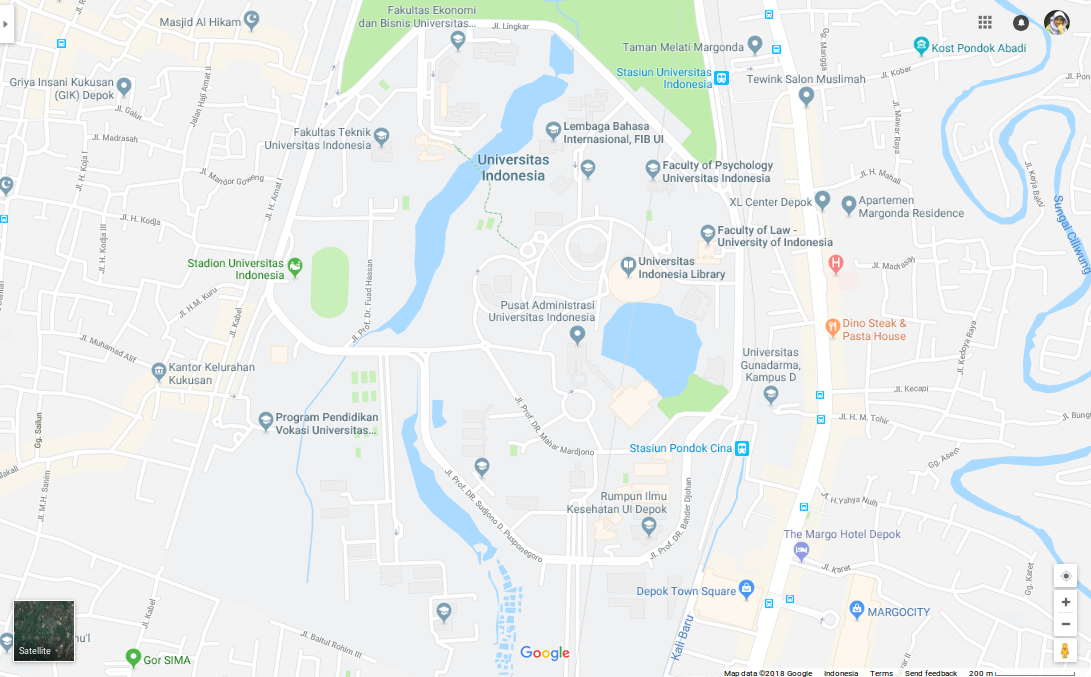
\includegraphics[width=12cm]{pics/ui.png}
	\caption{Peta Kampus Universitas Indonesia Depok}
	\label{fig:ui}
	\cite{ui.map}
\end{figure} 

Gambar di atas merupakan peta kampus {\ui}, Depok. Peta tersebut diambil dari Google Maps pada tanggal 21 Januari 2018 pukul 23:22. Peta tersebut berskala 1:100000.

Tidak semua wilayah dari kampus {\ui}, Depok dimasukkan dalam penelitian ini. Hanya wilayah sekitar fakultas dan stasiun tanpa memasukkan area asrama {\ui} dan area hutan {\ui}.

\section{Menggambarkan Demand dari \textit{Hotspot} Pada Peta}

Warna merah pada peta menggambarkan demand atau daerah yang harus dijangkau oleh \textit{hotspot} UI. Daerah yang digambarkan oleh warna merah tersebut adalah daerah-daerah dalam lingkungan fakultas, area publik, daerah-daerah penghubung antar fakultas, dan area pejalan kaki.

Area yang dipilih menjadi \textit{demand area} adalah daerah yang ramai dengan manusia seperti di stasiun, di halte bis kuning, di dalam bis kuning, perpustakaan, dan lain-lain.

\begin{figure}
	\centering
	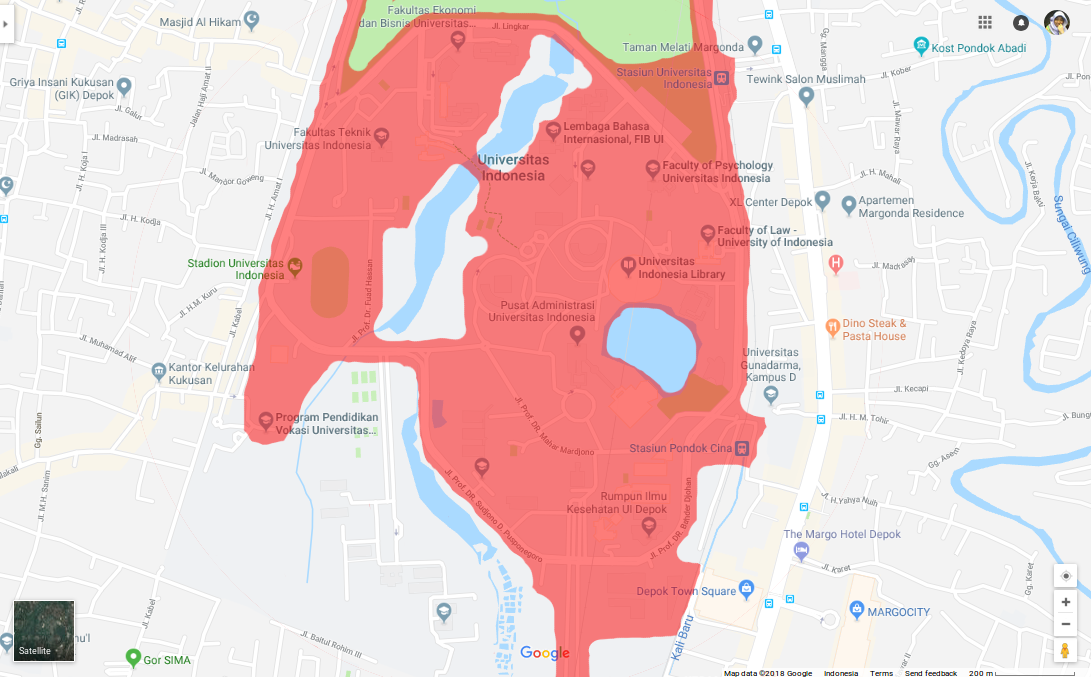
\includegraphics[width=14cm]{pics/ui-demand.png}
	\caption{Peta Kampus Universitas Indonesia dengan \textit{Demand} dari \textit{Hotspot}}
	\label{fig:uiDemand}
\end{figure} 

\section{Menambahkan Lokasi \textit{Hotspot} dan Bobot untuk Weighted Voronoi Diagram}

Berdasarkan data dari DSTI tentang lokasi \textit{access point} yang ada di kampus {\ui}, digambarkan setiap lokasi tersebut dalam peta kampus {\ui} Depok. Lokasi dari \textit{access point} digambarkan dengan titik berwarna hitam. Lokasi \textit{access point} yang digambarkan hanya \textit{access point} yang ada di lantai satu.

\begin{figure}
	\centering
	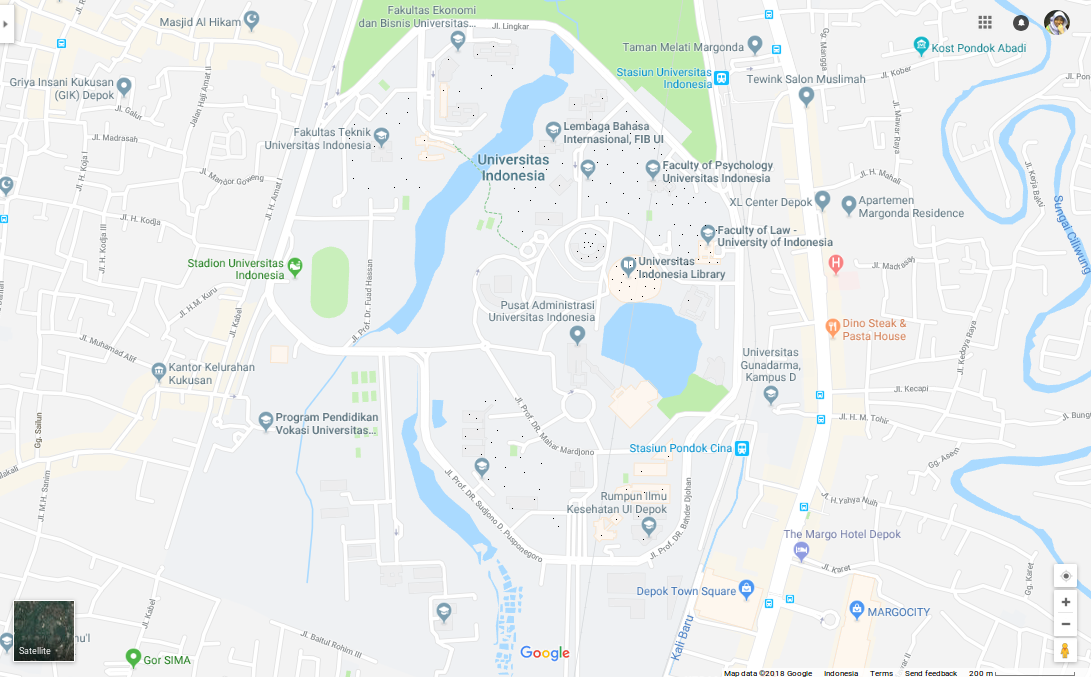
\includegraphics[width=14cm]{pics/ui-current.png}
	\caption{Peta Kampus Universitas Indonesia dengan Lokasi dari \textit{Hotspot} Saat Ini}
	\label{fig:uiCurrent}
\end{figure} 

Dalam \textit{Weighted Voronoi Diagram}, titik tersebut merupakan titik pusat dari diagram Voronoi. 

Setiap titik memiliki bobot masing-masing, yang mana bobot ini bergantung dari bandwidth dan kekuatan sinyal untuk masing-masing \textit{access point}. Bobot ini juga dihitung berdasarkan data \textit{access point} dari DSTI. 

Data \textit{access point} dari DSTI hanya menampilkan lokasi dari \textit{access point} beserta jenis \textit{router} yang digunakan, tanpa data mengenai \textit{bandwidth} dari setiap \textit{access point} tersebut. Sehingga untuk penelitian ini bobot yang digunakan hanya berdasarkan kekuatan sinyal dari setiap \textit{router}, dan \textit{bandwidth} untuk setiap \textit{router} dianggap sama.

\section{Menggambarkan Jangkauan \textit{Hotspot} pada Peta}

Dari setiap \textit{access point} digambarkan jangkauan dari \textit{access point} tersebut berupa lingkaran warna kuning. Panjang jari-jari dari lingkaran tersebut tergantung bobot dari titik pusatnya.

\begin{figure}
	\centering
	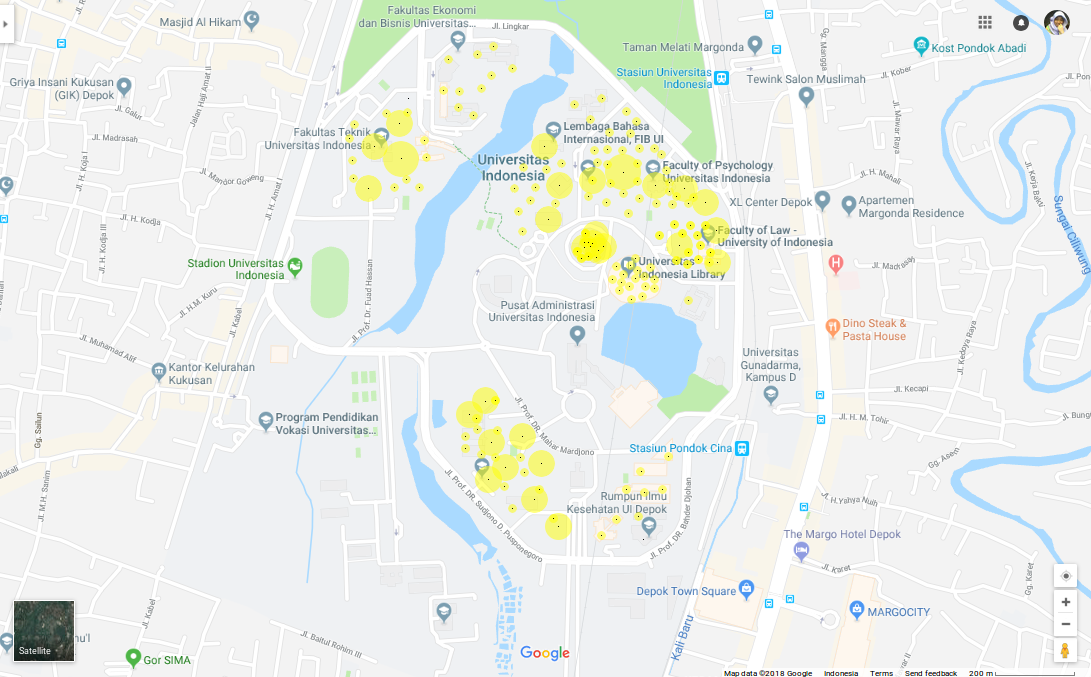
\includegraphics[width=14cm]{pics/ui-coverage.png}
	\caption{Peta Kampus Universitas Indonesia dengan Lokasi dari \textit{Hotspot} Saat Ini Beserta Jangkauannya}
	\label{fig:uiCoverage}
\end{figure} 

Untuk lingkaran yang \textit{overlapping} hal ini berarti daerah tersebut mendapatkan jangkauan dari lebih dari satu \textit{router}.

Jika peta jangkauan dari \textit{hotspot} kita terapkan pada peta \textit{demand} dari \textit{hotspot}, maka hasilnya sebagai berikut.

\begin{figure}
	\centering
	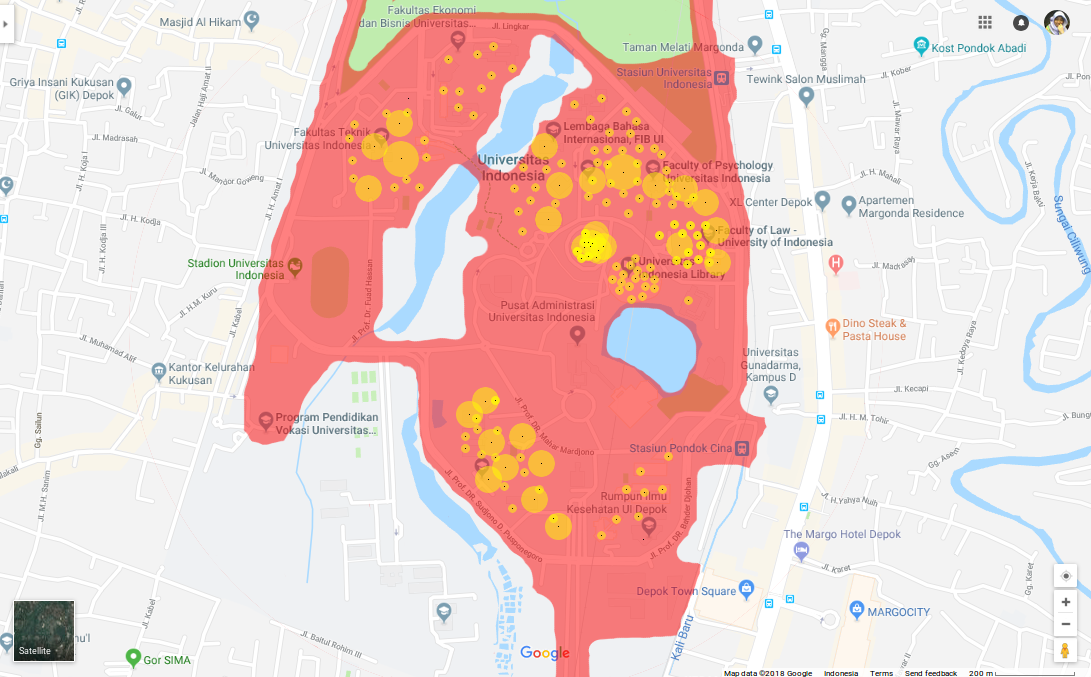
\includegraphics[width=14cm]{pics/ui-demand-coverage.png}
	\caption{Peta Kampus Universitas Indonesia dengan Lokasi dari \textit{Hotspot} Saat Ini Beserta Jangkauannya dan \textit{Demand} dari \textit{Hotspot}}
	\label{fig:uiCoverageDemand}
\end{figure} 

Dari gambar tersebut dapat kita lihat bahwa kondisi \textit{hotspot} saat ini masih belum memenuhi kebutuhan \textit{hotspot}.

\section{Menggambarkan Weighted Voronoi Diagram pada Peta}

Untuk melakukan penggambaran \textit{Weighted Voronoi Diagram} digunakan R Studio. Namun terdapat keterbatasan untuk penggambarannya yaitu gambar yang dihasilkan hanya berukuran 480x480 piksel. Dengan keterbatasan ini kemudian peta kampus {\ui} Depok dibagi menjadi beberapa bagian yang masing-masing bagiannya berukuran 480x480 piksel.

Untuk setiap bagian dalam peta, setiap lokasi dari \textit{access point} digambarkan ke dalam R studio berdasarkan lokasi koordinatnya. Setiap koordinat dari titik tersebut dituliskan dalam sebuah file yang kemudian akan dibaca oleh progam (sesuatu siapa namanya lupa).

Bobot untuk setiap titik tersebut juga disimpan dalam sebuah file berbeda. Nilai dari bobot tidak harus bilangan bulat, akan tetapi bisa berupa bilangan pecahan. 

Program tersebut kemudian melakukan \textit{plotting} dari data lokasi serta bobot dari setiap titik ke dalam gambar berukuran 480x480 piksel.

Setelah itu program ini akan menggambarkan \textit{Weighted Voronoi Diagram} dari kumpulan titik tersebut menjadi gambar ber-\textit{format} .jpeg.

Gambar \textit{Weighted Voronoi Diagram} yang dihasilkan dari program tersebut kemudian diubah menjadi gambar ber-\textit{format} .png menggunakan suatu aplikasi \textit{image converter} (link online). Gambar tersebut kemudian di \textit{overlay} pada gambar peta {\ui}.

Hal tersebut dilakukan untuk setiap potongan gambar dari peta {\ui} sehingga \textit{Weighted Voronoi Diagram} dari seluruh lokasi \textit{access point} tergambarkan dalam peta.

\section{Evaluasi Coverage \textit{Hotspot} Terhadap Demand}
Peta {\ui} yang sudah terdapat \textit{Weighted Voronoi Diagram} di dalamnya kemudian dievaluasi secara visual untuk mengetahui daerah mana yang belum mendapatkan jangkauan \textit{hotspot}.

Evaluasi yang dilakukan adalah dengan melihat apakah setiap daerah yang berwarna merah ada di dalam lingkaran berwarna kuning. Jika semua daerah yang berwarna merah sudah berada di dalam lingkaran berwarna kuning, maka setiap \textit{demand area} sudah mendapatkan jaringan hotspot. Namun jika ada daerah berwarna merah yang tidak berada dalam lingkaran berwarna kuning, maka perlu ditambahkan \textit{access point} baru di daerah tersebut.

\section{Menambahkan Lokasi \textit{Hotspot} Baru pada Daerah yang Belum Ter-cover Beserta Bobotnya}

Untuk daerah berwarna merah yang tidak berada pada lingkaran berwarna kuning, maka perlu ditambahkan titik baru atau \textit{access point} baru di dalamnya. Untuk menentukan di mana lokasi dari titik baru tersebut maka dilakukan analisis terhadap diagram Voronoi pada daerah tersebut. Lokasi baru dari \textit{access point} berada pada ujung diagram Voronoi, yang mana ujung diagram Voronoi adalah lokasi terjauh dari setiap titik-titik di sekitarnya. 

Hal tersebut dilakukan untuk setiap daerah berwarna merah yang tidak berada dalam lingkaran berwarna kuning. 

Setiap titik diberikan bobot yang sama dengan bobot terkecil diantara titik-titik yang ada. Hal ini ditujukan untuk mengambil seminimal mungkin \textit{cost} yang harus dikeluarkan untuk menambahkan \textit{access point} baru. 

\section{Menggambarkan Jangkauan untuk \textit{Hotspot} Baru pada Peta}

Untuk setiap titik baru yang ditambahkan dalam peta, kemudian digambarkan lingkaran kuning di sekitarnya yang menggambarkan jangkauan dari \textit{access point} tersebut seperti yang dilakukan dalam langkah sebelumnya.

\section{Menggambarkan Weighted Voronoi Diagram Baru}

Proses untuk menggambarkan \textit{Weighted Voronoi Diagram} sama dengan pada tahap sebelumnya. Dalam proses ini maka akan terbentuk diagram-diagram Voronoi baru, dan bentuk dari diagram-diagram Voronoi sebelumnya akan berubah. Hal ini dikarenakan...

\section{Evaluasi Coverage \textit{Hotspot} Baru Terhadap Demand}

Hasil dari pemetaan diagram Voronoi pada peta kemudian di-evaluasi kembali untuk mencari daerah mana yang belum mendapatkan jangkauan hotspot. Kemudian dilakukan hal yang sama sampai setiap daerah berwarna merah berada di dalam lingkaran-lingkaran berwarna kuning.

\section{Generate Weighted Voronoi Diagram}

Program tersebut menggambar suatu persegi yang berisi sepuluh titik berbobot yang lokasi dan bobotnya diambil secara random. Dari sepuluh titik berbobot itu kemudian digambarkan weighted voronoi diagramnya. \cite{voronoi.R}


\chapter{\babLima}

%-----------------------------------------------------------------------------%
\section{Kesimpulan}
%-----------------------------------------------------------------------------%



%-----------------------------------------------------------------------------%
\section{Saran}
%-----------------------------------------------------------------------------%

Penelitian ini dapat dikembangkan untuk pencarian distribusi \textit{hotspot} dalam ruang tiga dimensi. Sehingga persebaran jaringan tidak hanya ada pada bidang datar, tetapi juga bisa dalam bidang ruang. Misalnya untuk gedung-gedung yang terdiri dari beberapa lantai, jaringan yang terhalang oleh tembok, mempertimbangkan kontur tanah, dan lain-lain.

%\textit{Untuk next nya mungkin bisa dicari voronoi diagram di 3D. jadi kalo hotspot di lantai berapa tuh bisa tau juga range dalam bidang ruangnya. brarti kalo di 3D bedanya sih voronoi diagramnya bukan garis tapi bidang. dan untuk weighted voronoi diagram dia bisa berbentuk kurva juga. terus saran buat pengembangannya juga bisa diperhatikan kontur tanah dan gedung. bisa di-detect blank spotnya juga.}


%%-----------------------------------------------------------------------------%
\chapter{\babEnam}
%-----------------------------------------------------------------------------%

Bab ini menjelaskan tentang kesimpulan yang dapat diambil setelah melakukan implementasi untuk \textit{home automation gateway} serta saran  yang dapat penulis sampaikan untuk pengembangan sistem ini selanjutnya.

%-----------------------------------------------------------------------------%
\section{Kesimpulan}

%\textit{Gateway} dapat dibuat dengan menggunakan 

%Zigbee \textit{coordinator} dapat dihubungkan dengan \textit{gateway} dengan menggunakan sensor virtual yang ditanam dalam \textit{server} REST yang 

Dalam tugas akhir ini penulis berhasil mengimplementasikan sebuah \textit{gateway} yang dapat menghubungkan ZigBee \textit{coordinator} dengan \textit{cloud}. Setelah melakukan implementasi \textit{home automation gateway} dengan IoT \textit{cloud service} berbasis ZigBee \textit{network}, penulis dapat mengambil kesimpulan sebagai berikut.

\begin{enumerate}
\item \textit{Gateway} dapat dihubungkan dengan ZigBee \textit{coordinator} melalui REST API. Komunikasi antara \textit{gateway} dengan REST API dilakukan dengan menerjemahkan pesan dari \textit{client} menjadi perintah REST.

\item \textit{Gateway} dapat mengirimkan dan menerima data dari dan ke \textit{cloud} dengan menggunakan protokol MQTT. Pengiriman data dari \textit{gateway} ke \textit{cloud} dilakukan oleh MQTT \textit{client} yang berperan sebagai \textit{publisher}. Sedangkan penerimaan data dari \textit{cloud} ke \textit{gateway} dilakukan oleh MQTT \textit{client} yang berperan sebagai \textit{subscriber}.

\item Data tentang jaringan ZigBee disimpan dalam \textit{server} Mosquitto sehingga informasi tersebut dapat diakses dari mana saja melalui MQTT \textit{client}.

\item Berdasarkan beberapa percobaan yang telah dilakukan, \textit{gateway} telah berjalan dengan baik karena dapat mengendalikan perangkat lampu ZigBee melalui MQTT \textit{client}.

\end{enumerate}

\section{Saran}

Dari implementasi yang telah dilakukan penulis memiliki beberapa saran yang dapat digunakan untuk mengembangkan sistem ini.

\begin{enumerate}

\item Penggunaan protokol MQTT dapat disempurnakan dengan menyimpan \textit{client} yang pernah bergabung dalam jaringan dan topik yang pernah di-\textit{publish} atau di-\textit{subscribe} oleh \textit{client} tersebut. Hal ini ditujukan agar topik dan data dari \textit{client} tersebut masih tersedia dalam \textit{server} jika suatu saat \textit{client} bergabung kembali ke jaringan.

\item Perlu ditambahkan proses pendaftaran atau izin agar tidak semua \textit{client} dapat mengakses informasi atau mengubah keadaan dari jaringan ZigBee.

\item Pembacaan informasi tentang perangkat ZigBee dan pemberian perintah kepada perangkat ZigBee masih terhitung lambat, sehingga perlu dilakukan optimisasi agar proses yang dilakukan dapat berjalan lebih cepat.

\end{enumerate}


\printbibliography
%
% Daftar Pustaka
\include{pustaka}
%biblama (bukan biblatex)
\bibliography{bib}
%\bibliography{references}{}
%biblama (bukan biblatex)
%\bibliographystyle{alpha}
\bibliographystyle{ieeetr} 

%
% Lampiran 
%
\begin{appendix}
	%
% @author  Andreas Febrian
% @version 1.00 
% 
% Hanya sebuah pembatas bertuliskan LAMPIRAN ditengah halaman. 
% 

\begin{titlepage}
	\centering 
	\vspace*{6cm}
	\noindent \Huge{LAMPIRAN}
	\addChapter{LAMPIRAN}
\end{titlepage}
	\setcounter{page}{2}
	\include{lampiran}
\end{appendix}

\end{document}